\documentclass[12pt,a4paper]{report}

% ─── Packages ───────────────────────────────────────────────────────────────
\usepackage[margin=2.5cm]{geometry}
\usepackage[T1]{fontenc}
\usepackage[utf8]{inputenc}
\usepackage{newunicodechar}
% Map box-drawing and other non-T1 Unicode chars to safe ASCII equivalents
% (used in lstlisting code blocks and comments in this file)
\newunicodechar{─}{-}
\newunicodechar{│}{|}
\newunicodechar{├}{|}
\newunicodechar{└}{+}
\newunicodechar{•}{*}
\usepackage{lmodern}
\usepackage{microtype}
\usepackage{xcolor}
\usepackage{listings}
\usepackage{mdframed}
\usepackage{tcolorbox}
\tcbuselibrary{skins,breakable,listings}
\usepackage{hyperref}
\usepackage{graphicx}
\usepackage{booktabs}
\usepackage{tabularx}
\usepackage{enumitem}
\usepackage{titlesec}
\usepackage{fancyhdr}
\usepackage{amsmath}
\usepackage{amssymb}
\usepackage{tikz}
\usetikzlibrary{shapes.geometric, arrows.meta, positioning, fit, backgrounds}
\usepackage{forest}
\usepackage{multicol}
\usepackage{soul}
\usepackage{tocloft}
\usepackage{setspace}
\usepackage{parskip}
\usepackage{fontawesome5}
\setlength{\headheight}{14pt}

% ─── Colors ─────────────────────────────────────────────────────────────────
\definecolor{primaryblue}{HTML}{1A73E8}
\definecolor{darkblue}{HTML}{0D47A1}
\definecolor{lightblue}{HTML}{E3F2FD}
\definecolor{successgreen}{HTML}{2E7D32}
\definecolor{lightgreen}{HTML}{E8F5E9}
\definecolor{warnorange}{HTML}{E65100}
\definecolor{lightorange}{HTML}{FFF3E0}
\definecolor{dangerred}{HTML}{C62828}
\definecolor{lightred}{HTML}{FFEBEE}
\definecolor{codebg}{HTML}{F8F9FA}
\definecolor{codeborder}{HTML}{DEE2E6}
\definecolor{aicolor}{HTML}{6A0DAD}
\definecolor{ailight}{HTML}{F3E5F5}
\definecolor{handcolor}{HTML}{1B5E20}
\definecolor{handlight}{HTML}{F1F8E9}
\definecolor{commentgray}{HTML}{6C757D}
\definecolor{stringgreen}{HTML}{388E3C}
\definecolor{keywordblue}{HTML}{1565C0}
\definecolor{annotationpurple}{HTML}{7B1FA2}

% ─── Listings Style ──────────────────────────────────────────────────────────
\lstdefinestyle{javastyle}{
  language=Java,
  backgroundcolor=\color{codebg},
  basicstyle=\ttfamily\footnotesize,
  keywordstyle=\color{keywordblue}\bfseries,
  stringstyle=\color{stringgreen},
  commentstyle=\color{commentgray}\itshape,
  morecomment=[l]{//},
  morecomment=[s]{/*}{*/},
  emphstyle=\color{annotationpurple},
  emph={@Entity,@Table,@Id,@GeneratedValue,@Column,@OneToMany,@ManyToOne,
        @RestController,@GetMapping,@PostMapping,@PutMapping,@DeleteMapping,
        @RequestMapping,@RequestBody,@PathVariable,@Service,@Repository,
        @Autowired,@Component,@Configuration,@Bean,@EnableWebSecurity,
        @PreAuthorize,@Transactional,@Data,@NoArgsConstructor,@AllArgsConstructor,
        @Builder,@Getter,@Setter,@SpringBootApplication,@EnableJpaRepositories,
        @JoinColumn,@ManyToMany,@OneToOne,@Enumerated,@NotBlank,@NotNull,
        @Valid,@RequestParam,@ResponseStatus,@ExceptionHandler,@ControllerAdvice,
        @CrossOrigin,@EnableMethodSecurity,@GeneratedValue},
  numbers=left,
  numberstyle=\tiny\color{commentgray},
  stepnumber=1,
  numbersep=8pt,
  frame=single,
  framesep=4pt,
  rulecolor=\color{codeborder},
  tabsize=4,
  showstringspaces=false,
  breaklines=true,
  breakatwhitespace=false,
  captionpos=b,
  xleftmargin=15pt,
  xrightmargin=5pt,
}

\lstdefinestyle{xmlstyle}{
  language=XML,
  backgroundcolor=\color{codebg},
  basicstyle=\ttfamily\footnotesize,
  keywordstyle=\color{keywordblue},
  stringstyle=\color{stringgreen},
  commentstyle=\color{commentgray}\itshape,
  numbers=left,
  numberstyle=\tiny\color{commentgray},
  stepnumber=1,
  numbersep=8pt,
  frame=single,
  framesep=4pt,
  rulecolor=\color{codeborder},
  tabsize=2,
  showstringspaces=false,
  breaklines=true,
  captionpos=b,
  xleftmargin=15pt,
}

\lstdefinestyle{bashstyle}{
  language=bash,
  backgroundcolor=\color{codebg},
  basicstyle=\ttfamily\footnotesize,
  keywordstyle=\color{keywordblue}\bfseries,
  commentstyle=\color{commentgray}\itshape,
  numbers=none,
  frame=single,
  framesep=4pt,
  rulecolor=\color{codeborder},
  tabsize=2,
  showstringspaces=false,
  breaklines=true,
  captionpos=b,
  xleftmargin=5pt,
}

\lstdefinestyle{sqlstyle}{
  language=SQL,
  backgroundcolor=\color{codebg},
  basicstyle=\ttfamily\footnotesize,
  keywordstyle=\color{keywordblue}\bfseries,
  stringstyle=\color{stringgreen},
  commentstyle=\color{commentgray}\itshape,
  numbers=left,
  numberstyle=\tiny\color{commentgray},
  frame=single,
  framesep=4pt,
  rulecolor=\color{codeborder},
  tabsize=2,
  showstringspaces=false,
  breaklines=true,
  captionpos=b,
  xleftmargin=15pt,
}

\lstset{style=javastyle,
  extendedchars=true,
  literate={─}{-}1 {│}{|}1 {├}{|}1 {└}{+}1 {•}{*}1
           {←}{$\leftarrow$}1 {→}{$\rightarrow$}1
           {↑}{$\uparrow$}1 {↓}{$\downarrow$}1,
}

% ─── Custom Boxes ────────────────────────────────────────────────────────────
\tcbset{
  aibox/.style={
    enhanced, breakable,
    colback=ailight, colframe=aicolor,
    fonttitle=\bfseries\small,
    title={\faRobot\ AI CAN WRITE THIS},
    attach boxed title to top left={yshift=-2mm, xshift=5mm},
    boxed title style={colback=aicolor, colframe=aicolor, fontupper=\color{white}},
    top=6mm, left=4mm, right=4mm, bottom=4mm,
  },
  handbox/.style={
    enhanced, breakable,
    colback=handlight, colframe=handcolor,
    fonttitle=\bfseries\small,
    title={\faHandPaper\ WRITE THIS YOURSELF --- CRITICAL},
    attach boxed title to top left={yshift=-2mm, xshift=5mm},
    boxed title style={colback=handcolor, colframe=handcolor, fontupper=\color{white}},
    top=6mm, left=4mm, right=4mm, bottom=4mm,
  },
  notebox/.style={
    enhanced, breakable,
    colback=lightblue, colframe=primaryblue,
    fonttitle=\bfseries\small,
    title={\faBookOpen\ CONCEPT NOTE},
    attach boxed title to top left={yshift=-2mm, xshift=5mm},
    boxed title style={colback=primaryblue, colframe=primaryblue, fontupper=\color{white}},
    top=6mm, left=4mm, right=4mm, bottom=4mm,
  },
  warnbox/.style={
    enhanced, breakable,
    colback=lightorange, colframe=warnorange,
    fonttitle=\bfseries\small,
    title={\faExclamationTriangle\ WATCH OUT},
    attach boxed title to top left={yshift=-2mm, xshift=5mm},
    boxed title style={colback=warnorange, colframe=warnorange, fontupper=\color{white}},
    top=6mm, left=4mm, right=4mm, bottom=4mm,
  },
  successbox/.style={
    enhanced, breakable,
    colback=lightgreen, colframe=successgreen,
    fonttitle=\bfseries\small,
    title={\faCheckCircle\ CHECKPOINT},
    attach boxed title to top left={yshift=-2mm, xshift=5mm},
    boxed title style={colback=successgreen, colframe=successgreen, fontupper=\color{white}},
    top=6mm, left=4mm, right=4mm, bottom=4mm,
  },
  interviewbox/.style={
    enhanced, breakable,
    colback=lightred, colframe=dangerred,
    fonttitle=\bfseries\small,
    title={\faBullseye\ INTERVIEW GOLD},
    attach boxed title to top left={yshift=-2mm, xshift=5mm},
    boxed title style={colback=dangerred, colframe=dangerred, fontupper=\color{white}},
    top=6mm, left=4mm, right=4mm, bottom=4mm,
  },
}

% ─── Header / Footer ─────────────────────────────────────────────────────────
\pagestyle{fancy}
\fancyhf{}
\fancyhead[L]{\small\textcolor{commentgray}{FleetSync — Java Dev Guide}}
\fancyhead[R]{\small\textcolor{commentgray}{\leftmark}}
\fancyfoot[C]{\small\textcolor{commentgray}{\thepage}}
\renewcommand{\headrulewidth}{0.4pt}
\renewcommand{\footrulewidth}{0pt}

% ─── Section Styles ──────────────────────────────────────────────────────────
\titleformat{\chapter}[display]
  {\normalfont\huge\bfseries\color{darkblue}}
  {\chaptertitlename\ \thechapter}{20pt}{\Huge}
\titleformat{\section}
  {\normalfont\Large\bfseries\color{primaryblue}}
  {\thesection}{1em}{}
\titleformat{\subsection}
  {\normalfont\large\bfseries\color{darkblue}}
  {\thesubsection}{1em}{}
\titleformat{\subsubsection}
  {\normalfont\normalsize\bfseries\color{successgreen}}
  {\thesubsubsection}{1em}{}

% ─── Hyperref Setup ──────────────────────────────────────────────────────────
\hypersetup{
  colorlinks=true,
  linkcolor=primaryblue,
  urlcolor=primaryblue,
  citecolor=primaryblue,
  pdftitle={FleetSync: Complete Java Developer Guide},
  pdfauthor={Sheikh},
}

% ─── Helpers ─────────────────────────────────────────────────────────────────
\newcommand{\term}[1]{\textbf{\textcolor{primaryblue}{#1}}}
\newcommand{\code}[1]{\texttt{\textcolor{keywordblue}{#1}}}
\newcommand{\file}[1]{\texttt{\textcolor{successgreen}{#1}}}
\newcommand{\apipath}[1]{\texttt{\textcolor{dangerred}{#1}}}

% ─────────────────────────────────────────────────────────────────────────────
%  DOCUMENT START
% ─────────────────────────────────────────────────────────────────────────────
\begin{document}

% ─── Title Page ──────────────────────────────────────────────────────────────
\begin{titlepage}
  \centering
  \vspace*{1cm}

  {\fontsize{40}{48}\selectfont\bfseries\color{darkblue} FleetSync}\\[0.5cm]
  {\Large\color{primaryblue} Complete Java Developer Field Guide}\\[0.3cm]
  {\large\color{commentgray} From Zero to Junior Developer in 60 Days}\\[2cm]

  \begin{tcolorbox}[
    enhanced, width=12cm,
    colback=lightblue, colframe=primaryblue,
    boxrule=2pt, arc=8pt,
    left=10pt, right=10pt, top=10pt, bottom=10pt,
  ]
  \centering
  \large
  \textbf{Tech Stack:} Spring Boot 3 · MySQL · JWT · REST APIs\\[0.3cm]
  \textbf{Target:} Junior Java Developer / Internship\\[0.3cm]
  \textbf{Timeline:} 60 Days · 12 Weeks · MVP Ready\\[0.3cm]
  \textbf{Markets:} Pakistan · UAE · Remote
  \end{tcolorbox}

  \vspace{2cm}

  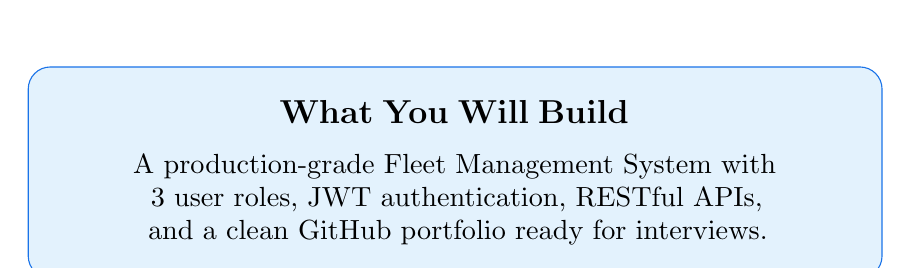
\begin{tikzpicture}
    \node[draw=primaryblue, fill=lightblue, rounded corners=8pt,
          inner sep=12pt, text width=10cm, align=center] {
      \textbf{\large What You Will Build}\\[6pt]
      A production-grade Fleet Management System with\\
      3 user roles, JWT authentication, RESTful APIs,\\
      and a clean GitHub portfolio ready for interviews.
    };
  \end{tikzpicture}

  \vfill

  {\color{commentgray}\small Built for Sheikh · 2024--2025 · Version 1.0}
\end{titlepage}

% ─── Table of Contents ───────────────────────────────────────────────────────
\tableofcontents
\newpage

% ─────────────────────────────────────────────────────────────────────────────
\chapter{How to Use This Guide}
% ─────────────────────────────────────────────────────────────────────────────

\section{The Mission}

You have 60 days. You want a job as a junior Java developer or intern. You have IntelliJ Ultimate (student plan), a project idea, and the motivation to make it happen. This guide turns that into a deployed, working project that gets you past screening calls.

Every chapter in this guide maps to one week of work. Every code block is explained line by line. Nothing is copy-paste-and-pray.

\section{The AI Policy in This Guide}

This is the most important section. Read it carefully.

\begin{tcolorbox}[aibox]
\textbf{AI-Writable Code} means: this code is boilerplate, configuration, or repetitive structure. A senior dev would also use AI or a template for this. You still need to \textbf{read and understand it}, but you do not need to memorise how to write it from scratch. Use GitHub Copilot, ChatGPT, or Claude to generate it. Then read every line and understand what it does before moving on.
\end{tcolorbox}

\begin{tcolorbox}[handbox]
\textbf{Write Yourself} means: this code is what interviewers test you on. If you cannot write this without AI, you will fail the technical interview. These are logic, structure, and design decisions that show you \textit{understand} Java and Spring Boot --- not just that you can prompt an AI. Do not skip these. Do not copy these. Write them yourself, make mistakes, fix them, and understand why they work.
\end{tcolorbox}

\begin{tcolorbox}[notebox]
\textbf{Concept Notes} explain \textit{why} something works the way it does. These are the answers to interview questions like ``explain how JWT works'' or ``what is the difference between authentication and authorization?''
\end{tcolorbox}

\begin{tcolorbox}[interviewbox]
\textbf{Interview Gold} boxes contain exact talking points, common questions, and what UAE/Pakistan recruiters actually ask for this topic. Memorise these.
\end{tcolorbox}

\section{Box Color Legend Summary}

\begin{tabularx}{\textwidth}{@{}llX@{}}
\toprule
\textbf{Color} & \textbf{Type} & \textbf{Meaning} \\
\midrule
Purple & AI Can Write This & Boilerplate/config. Generate + understand. \\
Green & Write Yourself & Core logic. Write from scratch. Interview material. \\
Blue & Concept Note & Theory behind the code. \\
Orange & Watch Out & Common mistakes beginners make. \\
Light Green & Checkpoint & Verify your progress before moving on. \\
Red & Interview Gold & What recruiters will ask you. \\
\bottomrule
\end{tabularx}

\section{Tools You Need (Install Now)}

\begin{enumerate}[leftmargin=2cm]
  \item \textbf{IntelliJ IDEA Ultimate} --- You already have this (student plan). Make sure it is the latest version.
  \item \textbf{Java 17 (Temurin/OpenJDK)} --- Download from \href{https://adoptium.net}{adoptium.net}. In terminal: \code{java -version} should say 17.
  \item \textbf{XAMPP} --- For local MySQL. Download from \href{https://apachefriends.org}{apachefriends.org}. Start the MySQL module.
  \item \textbf{Postman} --- For testing your APIs. Download from \href{https://postman.com}{postman.com}.
  \item \textbf{Git} --- \code{git --version} in terminal. If not installed: \href{https://git-scm.com}{git-scm.com}.
  \item \textbf{GitHub Account} --- Create one if you do not have it. This is your portfolio.
\end{enumerate}

\begin{tcolorbox}[successbox]
Run these commands in your terminal before proceeding:
\begin{lstlisting}[style=bashstyle]
java -version     # Should say: openjdk version "17.x.x"
git --version     # Should say: git version 2.x.x
mysql --version   # Start XAMPP MySQL first, then test
\end{lstlisting}
All three should return version numbers without errors. If any fail, fix it before starting Chapter 2.
\end{tcolorbox}

% ─────────────────────────────────────────────────────────────────────────────
\chapter{Understanding FleetSync — What You Are Building}
% ─────────────────────────────────────────────────────────────────────────────

\section{The Real-World Problem}

Companies like TCS Pakistan, Leopard Courier, Careem, and Aramex manage hundreds to thousands of vehicles. They need software to:

\begin{itemize}
  \item Know which vehicle is assigned to which driver
  \item Know which driver is on which trip right now
  \item Let managers see everything and drivers see only their own data
  \item Keep track of trip history for payroll and performance
\end{itemize}

This is what you are building. It is a real problem, not a todo list.

\section{System Roles}

FleetSync has exactly three types of users. Understanding these roles before writing a single line of code is critical.

\begin{tcolorbox}[notebox]
\textbf{RBAC --- Role-Based Access Control.} A security pattern where what you can do in a system is determined by your \textit{role}, not by who you are individually. In FleetSync: your role is ADMIN, MANAGER, or DRIVER. Each role has a defined set of permissions. This is the industry standard for enterprise systems. Spring Security implements RBAC via \code{@PreAuthorize} annotations.
\end{tcolorbox}

\subsection{Role: ADMIN}
\begin{itemize}
  \item Creates user accounts
  \item Assigns roles to users
  \item Can deactivate or delete users
  \item \textbf{Cannot} manage fleets or trips (that is the manager's job)
\end{itemize}

\subsection{Role: MANAGER}
\begin{itemize}
  \item Full CRUD on vehicles (trucks, bikes, ships, taxis)
  \item Full CRUD on drivers
  \item Creates and manages trips
  \item Assigns drivers to trips
  \item Views all dashboards and reports
\end{itemize}

\subsection{Role: DRIVER}
\begin{itemize}
  \item Views only his own assigned trips
  \item Marks a trip as ``In Progress'' or ``Completed''
  \item Views his own profile
  \item Cannot see any other driver's data
\end{itemize}

\section{The Five Modules}

\begin{tabularx}{\textwidth}{@{}lXl@{}}
\toprule
\textbf{Module} & \textbf{What it does} & \textbf{Week} \\
\midrule
Auth Module & Register, login, JWT token issue, role assignment & Week 7--8 \\
Fleet Module & CRUD for all vehicle types & Week 5--6 \\
Driver Module & CRUD for drivers, assignment & Week 5--6 \\
Trip Module & Create trips, assign driver+vehicle, lifecycle & Week 9 \\
User Module & Admin-level user management & Week 8 \\
\bottomrule
\end{tabularx}

\section{Complete Entity Relationship Overview}

Before writing code, you must understand how the data connects. This is called a \term{Database Schema} or \term{Entity Relationship Diagram (ERD)}.

\begin{figure}[h!]
\centering
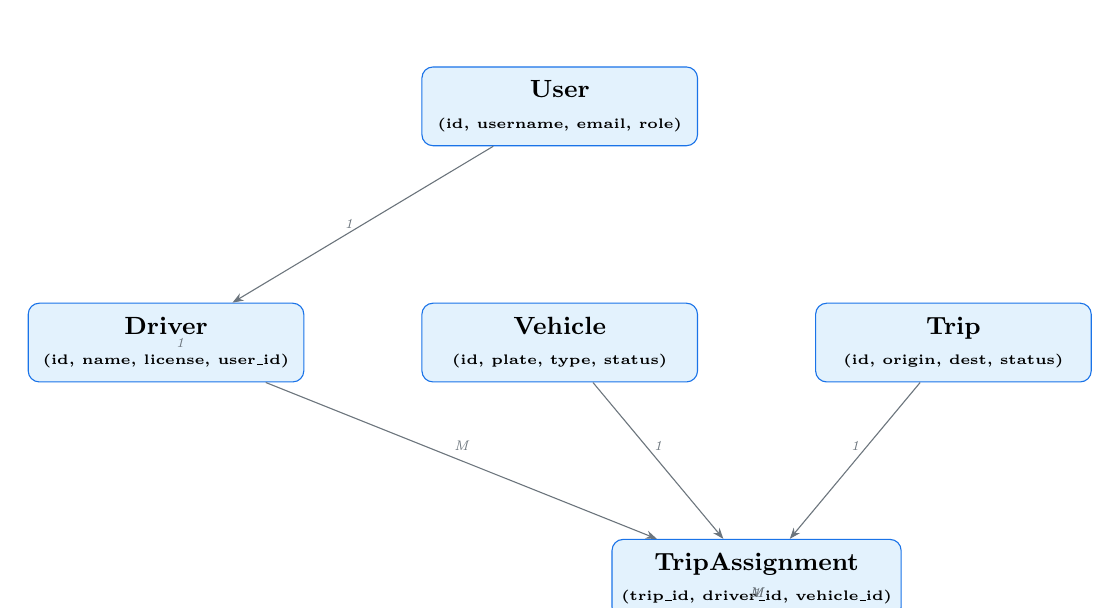
\begin{tikzpicture}[
  entity/.style={draw=primaryblue, fill=lightblue, rounded corners=4pt,
                  minimum width=3.5cm, minimum height=1cm, align=center,
                  font=\bfseries\small},
  relation/.style={draw=commentgray, -{Stealth[length=4pt]}},
  label/.style={font=\tiny\itshape\color{commentgray}},
]

\node[entity] (user) at (0,0) {User\\\tiny(id, username, email, role)};
\node[entity] (driver) at (-5,-3) {Driver\\\tiny(id, name, license, user\_id)};
\node[entity] (vehicle) at (0,-3) {Vehicle\\\tiny(id, plate, type, status)};
\node[entity] (trip) at (5,-3) {Trip\\\tiny(id, origin, dest, status)};
\node[entity] (tripdriver) at (2.5,-6) {TripAssignment\\\tiny(trip\_id, driver\_id, vehicle\_id)};

\draw[relation] (user) -- node[label,left]{1} (driver) node[label,right]{1};
\draw[relation] (driver) -- node[label,above]{M} (tripdriver) node[label,below]{1};
\draw[relation] (vehicle) -- node[label,above]{1} (tripdriver) node[label,below]{M};
\draw[relation] (trip) -- node[label,above]{1} (tripdriver) node[label,below]{M};

\end{tikzpicture}
\caption{FleetSync Entity Relationship Diagram}
\end{figure}

\section{API Structure Overview}

Here is every endpoint you will build. This is your north star --- everything in the next 10 weeks is building toward this list.

\subsection{Auth APIs}
\begin{tabularx}{\textwidth}{@{}llX@{}}
\toprule
\textbf{Method} & \textbf{Endpoint} & \textbf{Description} \\
\midrule
POST & \apipath{/api/auth/register} & Register a new user \\
POST & \apipath{/api/auth/login} & Login, receive JWT token \\
POST & \apipath{/api/auth/logout} & Logout (client-side token drop) \\
\bottomrule
\end{tabularx}

\subsection{Fleet/Vehicle APIs}
\begin{tabularx}{\textwidth}{@{}llX@{}}
\toprule
\textbf{Method} & \textbf{Endpoint} & \textbf{Description} \\
\midrule
GET & \apipath{/api/vehicles} & Get all vehicles (MANAGER) \\
GET & \apipath{/api/vehicles/\{id\}} & Get vehicle by ID (MANAGER) \\
POST & \apipath{/api/vehicles} & Create new vehicle (MANAGER) \\
PUT & \apipath{/api/vehicles/\{id\}} & Update vehicle (MANAGER) \\
DELETE & \apipath{/api/vehicles/\{id\}} & Delete vehicle (MANAGER) \\
GET & \apipath{/api/vehicles/type/\{type\}} & Filter by type (MANAGER) \\
\bottomrule
\end{tabularx}

\subsection{Driver APIs}
\begin{tabularx}{\textwidth}{@{}llX@{}}
\toprule
\textbf{Method} & \textbf{Endpoint} & \textbf{Description} \\
\midrule
GET & \apipath{/api/drivers} & Get all drivers (MANAGER) \\
GET & \apipath{/api/drivers/\{id\}} & Get driver by ID \\
POST & \apipath{/api/drivers} & Create driver (MANAGER) \\
PUT & \apipath{/api/drivers/\{id\}} & Update driver (MANAGER) \\
DELETE & \apipath{/api/drivers/\{id\}} & Delete driver (MANAGER) \\
GET & \apipath{/api/drivers/\{id\}/trips} & Driver trip history \\
\bottomrule
\end{tabularx}

\subsection{Trip APIs}
\begin{tabularx}{\textwidth}{@{}llX@{}}
\toprule
\textbf{Method} & \textbf{Endpoint} & \textbf{Description} \\
\midrule
GET & \apipath{/api/trips} & All trips (MANAGER) \\
GET & \apipath{/api/trips/\{id\}} & Trip detail \\
POST & \apipath{/api/trips} & Create trip (MANAGER) \\
PUT & \apipath{/api/trips/\{id\}/start} & Start trip (DRIVER/MANAGER) \\
PUT & \apipath{/api/trips/\{id\}/complete} & Complete trip (DRIVER/MANAGER) \\
GET & \apipath{/api/trips/my-trips} & Driver's own trips (DRIVER) \\
\bottomrule
\end{tabularx}

% ─────────────────────────────────────────────────────────────────────────────
\chapter{Week 1--2: Java Refresher + Spring Boot Basics}
% ─────────────────────────────────────────────────────────────────────────────

\section{Week Goals}

By the end of Week 2, you will have:
\begin{itemize}
  \item A running Spring Boot project that responds to HTTP requests
  \item A ``Hello FleetSync'' endpoint working in Postman
  \item Understanding of how Spring Boot starts and why
  \item Your first Git commit pushed to GitHub
\end{itemize}

\section{Java Concepts You Must Refresh}

Before touching Spring Boot, make sure these Java concepts are solid. If any feel shaky, spend one day on them before starting.

\begin{tcolorbox}[handbox]
\textbf{Do not use AI for these.} These are core Java --- interviewers test these directly.

\begin{itemize}
  \item \textbf{Classes and Objects} --- What is a class? What is an object? How do you instantiate?
  \item \textbf{Interfaces} --- What does \code{implements} mean? Why use an interface?
  \item \textbf{Inheritance} --- \code{extends} keyword, method overriding, \code{super}
  \item \textbf{Access Modifiers} --- \code{public}, \code{private}, \code{protected}, package-private
  \item \textbf{Collections} --- \code{List}, \code{ArrayList}, \code{HashMap}. Know the difference.
  \item \textbf{Exception Handling} --- \code{try-catch-finally}, checked vs unchecked exceptions
  \item \textbf{Generics} --- \code{List<String>}, \code{Optional<T>}. What is the \code{<T>}?
\end{itemize}
\end{tcolorbox}

\begin{tcolorbox}[interviewbox]
The most common Java basics question in junior interviews: ``What is the difference between \code{ArrayList} and \code{LinkedList}?''\\[6pt]
\textbf{Answer:} ArrayList is backed by a dynamic array. Random access is $O(1)$. Insertion/deletion in the middle is $O(n)$ because elements shift. LinkedList is backed by a doubly-linked chain of nodes. Access is $O(n)$ but insertion/deletion at known positions is $O(1)$. For most Spring Boot use cases (iterating a list from DB), ArrayList is preferred.
\end{tcolorbox}

\section{Creating the Spring Boot Project}

\begin{tcolorbox}[aibox]
Go to \href{https://start.spring.io}{start.spring.io}. This tool generates the project skeleton. A senior dev also uses this. You do not hand-write Maven \code{pom.xml} from scratch.
\end{tcolorbox}

Configure it exactly like this:

\begin{lstlisting}[style=bashstyle,caption=Spring Initializr Settings]
Project:      Maven
Language:     Java
Spring Boot:  3.4.x   (latest stable 3.x)
Packaging:    Jar
Java:         17

Group:        com.fleetsync
Artifact:     fleetsync
Name:         fleetsync
Package name: com.fleetsync
Description:  Fleet Management System

Dependencies:
  - Spring Web
  - Spring Data JPA
  - MySQL Driver
  - Lombok
  - Spring Security
  - Spring Boot DevTools
\end{lstlisting}

Click \textbf{Generate}, download the zip, extract it, and open it in IntelliJ.

\section{Understanding the Generated Project Structure}

\begin{tcolorbox}[notebox]
\textbf{Maven} is a build tool. Think of it as npm but for Java. Your \file{pom.xml} is like \file{package.json} --- it declares your project's dependencies (libraries) and how to build the project. When IntelliJ opens your project, it reads \file{pom.xml} and automatically downloads all the declared libraries.
\end{tcolorbox}

Here is what Spring Initializr generated and what every file means:

\begin{lstlisting}[style=bashstyle,caption=Project Structure After Generation]
fleetsync/
├── src/
│   ├── main/
│   │   ├── java/
│   │   │   └── com/fleetsync/
│   │   │       └── FleetsyncApplication.java   <- Entry point
│   │   └── resources/
│   │       ├── application.properties           <- Config file
│   │       ├── static/                          <- Static files (empty for now)
│   │       └── templates/                       <- Templates (empty for now)
│   └── test/
│       └── java/
│           └── com/fleetsync/
│               └── FleetsyncApplicationTests.java
├── pom.xml                                      <- Maven config (dependencies)
└── .gitignore
\end{lstlisting}

\subsection{The Entry Point: FleetsyncApplication.java}

\begin{tcolorbox}[handbox]
Open \file{FleetsyncApplication.java}. Read it. You will see this:
\end{tcolorbox}

\begin{lstlisting}[caption=FleetsyncApplication.java -- The Entry Point]
package com.fleetsync;

import org.springframework.boot.SpringApplication;
import org.springframework.boot.autoconfigure.SpringBootApplication;

@SpringBootApplication  // (1)
public class FleetsyncApplication {

    public static void main(String[] args) {
        SpringApplication.run(FleetsyncApplication.class, args);  // (2)
    }
}
\end{lstlisting}

\textbf{Line-by-line explanation:}

\begin{enumerate}
  \item \code{@SpringBootApplication} is actually three annotations in one:
    \begin{itemize}
      \item \code{@Configuration} --- This class can define beans (objects Spring manages)
      \item \code{@EnableAutoConfiguration} --- Spring automatically configures things based on what jars are on the classpath (e.g., it sees you have MySQL driver, so it sets up a database connection)
      \item \code{@ComponentScan} --- Spring scans all classes in \code{com.fleetsync} and sub-packages for annotations like \code{@Service}, \code{@Repository}, \code{@RestController} and registers them
    \end{itemize}
  \item \code{SpringApplication.run()} starts the embedded Tomcat server (yes, Spring Boot has a web server \textit{built in} --- no need to deploy a WAR file to external Tomcat)
\end{enumerate}

\begin{tcolorbox}[notebox]
\textbf{What is an Annotation in Java?} An annotation starts with \code{@}. It is metadata --- extra information attached to a class, method, or field that tells the framework (Spring) how to treat that element. When you write \code{@RestController}, you are telling Spring: ``This class handles HTTP requests. Register it as a controller.'' Without the annotation, Spring ignores the class.
\end{tcolorbox}

\section{Configuring the Database Connection}

Open \file{src/main/resources/application.properties} and configure it:

\begin{tcolorbox}[aibox]
This configuration block is boilerplate. Use the one below exactly. You will understand each property from the comments.
\end{tcolorbox}

\begin{lstlisting}[style=xmlstyle,caption=application.properties -- Full Database Configuration]
# ── Application Name ──────────────────────────────────────────────────────────
spring.application.name=fleetsync

# ── Database Connection ────────────────────────────────────────────────────────
# URL format: jdbc:mysql://host:port/database_name?options
spring.datasource.url=jdbc:mysql://localhost:3306/fleetsync_db?useSSL=false&serverTimezone=UTC&allowPublicKeyRetrieval=true
spring.datasource.username=root
spring.datasource.password=          # Leave blank if XAMPP MySQL has no password
spring.datasource.driver-class-name=com.mysql.cj.jdbc.Driver

# ── JPA / Hibernate ───────────────────────────────────────────────────────────
# hibernate.ddl-auto options:
# create       -> drops all tables and recreates every restart (use in early dev)
# create-drop  -> creates tables on start, drops on stop
# update       -> updates schema if entities change (use in mid dev)
# validate     -> validates schema matches entities, throws error if not
# none         -> does nothing (use in production)
spring.jpa.hibernate.ddl-auto=update

# Show SQL queries in console (great for learning what JPA generates)
spring.jpa.show-sql=true
spring.jpa.properties.hibernate.format_sql=true

# MySQL dialect tells Hibernate what SQL syntax to use
spring.jpa.properties.hibernate.dialect=org.hibernate.dialect.MySQL8Dialect

# ── Server Port ───────────────────────────────────────────────────────────────
server.port=8080

# ── Logging ───────────────────────────────────────────────────────────────────
logging.level.com.fleetsync=DEBUG
logging.level.org.springframework.security=DEBUG
\end{lstlisting}

\textbf{Now create the database in XAMPP:}

\begin{lstlisting}[style=sqlstyle,caption=Create the database in MySQL]
-- Open phpMyAdmin (http://localhost/phpmyadmin)
-- Or use MySQL terminal:
CREATE DATABASE fleetsync_db;
USE fleetsync_db;
-- You do NOT need to create tables manually.
-- JPA/Hibernate will create them automatically from your @Entity classes.
\end{lstlisting}

\section{Your First REST Controller}

This is where Spring Boot becomes real. You will create an endpoint that returns text when you call it via HTTP.

\begin{tcolorbox}[handbox]
Write this yourself. This is the most fundamental Spring Boot pattern. You will write this kind of class 15 more times in this project. Muscle memory matters here.
\end{tcolorbox}

Create a new package \file{com.fleetsync.controller} and inside it create \file{TestController.java}:

\begin{lstlisting}[caption=TestController.java -- Your First REST Endpoint]
package com.fleetsync.controller;

import org.springframework.web.bind.annotation.GetMapping;
import org.springframework.web.bind.annotation.RequestMapping;
import org.springframework.web.bind.annotation.RestController;

@RestController                     // (1) Marks this as a REST controller
@RequestMapping("/api/test")        // (2) All endpoints in this class start with /api/test
public class TestController {

    @GetMapping("/hello")           // (3) Handles GET /api/test/hello
    public String hello() {
        return "Hello FleetSync! Your Spring Boot app is running.";
    }

    @GetMapping("/status")          // (4) Handles GET /api/test/status
    public String status() {
        return "FleetSync API Status: UP";
    }
}
\end{lstlisting}

\textbf{Line-by-line:}

\begin{enumerate}
  \item \code{@RestController} = \code{@Controller} + \code{@ResponseBody}. It means: this class handles HTTP requests AND the return value of each method is written directly to the HTTP response body (as JSON or plain text). Without \code{@ResponseBody}, Spring would try to find a view template to render.
  \item \code{@RequestMapping("/api/test")} sets the \textit{base URL} for all methods in this class. Every method's URL is this base plus the method's own mapping.
  \item \code{@GetMapping("/hello")} maps HTTP GET requests to \code{/api/test/hello} to this method.
  \item The full URL becomes \code{http://localhost:8080/api/test/status}
\end{enumerate}

\begin{tcolorbox}[warnbox]
If you run the app now and call \code{http://localhost:8080/api/test/hello} in Postman, you will get a \textbf{401 Unauthorized} error. Why? Because you added \code{Spring Security} as a dependency. By default, Spring Security blocks every request. We will temporarily disable it for testing, then configure it properly in Week 7.
\end{tcolorbox}

\subsection{Temporarily Disable Security for Testing}

Create \file{com.fleetsync.config.SecurityConfig.java}:

\begin{lstlisting}[caption=SecurityConfig.java -- Temporary Open Security for Development]
package com.fleetsync.config;

import org.springframework.context.annotation.Bean;
import org.springframework.context.annotation.Configuration;
import org.springframework.security.config.annotation.web.builders.HttpSecurity;
import org.springframework.security.config.annotation.web.configuration.EnableWebSecurity;
import org.springframework.security.web.SecurityFilterChain;

@Configuration
@EnableWebSecurity
public class SecurityConfig {

    @Bean
    public SecurityFilterChain securityFilterChain(HttpSecurity http) throws Exception {
        http
            .csrf(csrf -> csrf.disable())   // Disable CSRF for REST APIs (stateless)
            .authorizeHttpRequests(auth -> auth
                .anyRequest().permitAll()   // Allow ALL requests for now (development only)
            );
        return http.build();
    }
}
\end{lstlisting}

\begin{tcolorbox}[warnbox]
\code{.anyRequest().permitAll()} means anyone can call any endpoint. This is \textbf{ONLY} for development. In Week 7, you will replace this with proper JWT-based security. If you deploy with this config, your app has zero security.
\end{tcolorbox}

\section{Running the App and Testing in Postman}

\begin{enumerate}
  \item In IntelliJ, click the green Run button or press \textbf{Shift+F10}
  \item Watch the console for: \code{Tomcat started on port(s): 8080}
  \item Open Postman
  \item Create a new GET request to: \code{http://localhost:8080/api/test/hello}
  \item Send --- you should see: \code{Hello FleetSync! Your Spring Boot app is running.}
\end{enumerate}

\begin{tcolorbox}[successbox]
\textbf{Week 1--2 Checkpoint:}
\begin{itemize}
  \item[$\checkmark$] Spring Boot app starts without errors
  \item[$\checkmark$] \code{/api/test/hello} returns a response in Postman
  \item[$\checkmark$] \code{/api/test/status} returns a response in Postman
  \item[$\checkmark$] Project is pushed to a GitHub repository (\code{git init}, \code{git add .}, \code{git commit}, \code{git push})
\end{itemize}
If any of these fail, fix before proceeding to Week 3.
\end{tcolorbox}

\section{Setting Up Git from Day One}

\begin{lstlisting}[style=bashstyle,caption=Initial Git Setup]
# In your project folder (terminal):
git init
git add .
git commit -m "feat: initial Spring Boot project setup"

# Create a repo on GitHub (fleetsync), then:
git remote add origin https://github.com/YOUR_USERNAME/fleetsync.git
git branch -M main
git push -u origin main
\end{lstlisting}

\begin{tcolorbox}[notebox]
\textbf{Commit Message Convention:} Use \textbf{Conventional Commits} format. This is what every professional team uses.
\begin{itemize}
  \item \code{feat:} --- New feature
  \item \code{fix:} --- Bug fix
  \item \code{refactor:} --- Code restructure, no logic change
  \item \code{docs:} --- Documentation update
  \item \code{chore:} --- Config, build, tools
\end{itemize}
Example: \code{feat: add vehicle CRUD endpoints}. Recruiters check your commit history. Clean commits look professional.
\end{tcolorbox}

% ─────────────────────────────────────────────────────────────────────────────
\chapter{Week 3--4: Database Layer (JPA, Entities, Repositories)}
% ─────────────────────────────────────────────────────────────────────────────

\section{Week Goals}

By end of Week 4, you will have:
\begin{itemize}
  \item All five Entity classes defined and mapped to MySQL tables
  \item JPA automatically creating your database tables
  \item Repository interfaces for each entity
  \item Understanding of JPA relationships (OneToMany, ManyToOne)
\end{itemize}

\section{What is JPA and Hibernate?}

\begin{tcolorbox}[notebox]
\textbf{JPA (Java Persistence API)} is a specification (a set of rules/interfaces) that defines how Java objects should be stored in relational databases. It is not a library itself --- it is a contract.

\textbf{Hibernate} is the most popular \textit{implementation} of JPA. When you use \code{@Entity}, \code{@Table}, \code{@OneToMany} etc., you are using JPA annotations, but Hibernate is the engine doing the actual database work under the hood.

\textbf{The key idea --- ORM (Object Relational Mapping):} Instead of writing SQL like \code{INSERT INTO vehicles VALUES (...)}, you write Java code like \code{vehicleRepository.save(vehicle)} and JPA/Hibernate generates the SQL for you.

\textbf{Tradeoff:} ORM is faster to develop with but can generate inefficient SQL. Senior devs know when to bypass JPA and write raw SQL (called JPQL or native queries). You will learn this later.
\end{tcolorbox}

\section{Package Structure}

Create this package structure in IntelliJ now:

\begin{lstlisting}[style=bashstyle,caption=FleetSync Package Structure]
com.fleetsync/
├── config/          # Security, CORS, JWT config
├── controller/      # REST controllers (@RestController)
├── service/         # Business logic (@Service)
├── repository/      # Database access (@Repository)
├── entity/          # Database tables (@Entity)
├── dto/             # Data Transfer Objects (request/response shapes)
├── exception/       # Custom exceptions and error handlers
├── security/        # JWT filter, UserDetails, etc.
└── enums/           # Enum types (VehicleType, TripStatus, Role)
\end{lstlisting}

\begin{tcolorbox}[notebox]
\textbf{Why separate packages?} This is \textbf{Layered Architecture} (also called N-Tier Architecture). Each layer has one responsibility:
\begin{itemize}
  \item \textbf{Controller} layer: receives HTTP request, validates input, calls service, returns response
  \item \textbf{Service} layer: contains business logic, calls repository, throws business exceptions
  \item \textbf{Repository} layer: talks to the database only --- no business logic here
  \item \textbf{Entity} layer: represents database tables as Java objects
\end{itemize}
This separation makes code maintainable and testable. It is what every professional Java project uses.
\end{tcolorbox}

\section{Creating Enums First}

Enums define fixed sets of values. Create these in the \code{enums} package:

\begin{tcolorbox}[handbox]
These are simple but important. Write them yourself. They define the domain language of your entire system.
\end{tcolorbox}

\begin{lstlisting}[caption=VehicleType.java]
package com.fleetsync.enums;

public enum VehicleType {
    TRUCK,
    BIKE,
    SHIP,
    TAXI,
    VAN
}
\end{lstlisting}

\begin{lstlisting}[caption=VehicleStatus.java]
package com.fleetsync.enums;

public enum VehicleStatus {
    AVAILABLE,      // Ready to be assigned
    ON_TRIP,        // Currently on a trip
    MAINTENANCE,    // Under repair
    RETIRED         // No longer in service
}
\end{lstlisting}

\begin{lstlisting}[caption=TripStatus.java]
package com.fleetsync.enums;

public enum TripStatus {
    PENDING,        // Created but driver hasn't started yet
    IN_PROGRESS,    // Driver has started the trip
    COMPLETED,      // Trip finished successfully
    CANCELLED       // Trip was cancelled
}
\end{lstlisting}

\begin{lstlisting}[caption=Role.java]
package com.fleetsync.enums;

public enum Role {
    ADMIN,
    MANAGER,
    DRIVER
}
\end{lstlisting}

\section{The User Entity}

\begin{tcolorbox}[handbox]
Write this yourself. The User entity is the centerpiece of your entire auth system. Every annotation here will be tested in interviews. Understand what each one does.
\end{tcolorbox}

\begin{lstlisting}[caption=User.java -- The User Entity]
package com.fleetsync.entity;

import com.fleetsync.enums.Role;
import jakarta.persistence.*;
import lombok.AllArgsConstructor;
import lombok.Builder;
import lombok.Data;
import lombok.NoArgsConstructor;
import java.time.LocalDateTime;

@Entity                         // (1) Marks this class as a JPA entity (maps to DB table)
@Table(name = "users")          // (2) Table name in MySQL (avoids conflict with SQL keyword 'user')
@Data                           // (3) Lombok: generates getters, setters, equals, hashCode, toString
@Builder                        // (4) Lombok: generates a builder pattern for object creation
@NoArgsConstructor              // (5) Lombok: generates empty constructor (required by JPA)
@AllArgsConstructor             // (6) Lombok: generates constructor with all fields
public class User {

    @Id                                         // (7) This field is the primary key
    @GeneratedValue(strategy = GenerationType.IDENTITY)  // (8) Auto-increment by DB
    private Long id;

    @Column(unique = true, nullable = false, length = 50)
    private String username;                    // (9) Must be unique, cannot be null

    @Column(unique = true, nullable = false)
    private String email;

    @Column(nullable = false)
    private String password;                    // Will store HASHED password, never plain text

    @Enumerated(EnumType.STRING)               // (10) Store enum as STRING in DB (not as number)
    @Column(nullable = false)
    private Role role;

    @Column(nullable = false)
    private Boolean isActive = true;

    @Column(updatable = false)                 // (11) Set on creation, never updated
    private LocalDateTime createdAt;

    private LocalDateTime updatedAt;

    @PrePersist                                // (12) Called automatically before INSERT
    protected void onCreate() {
        createdAt = LocalDateTime.now();
        updatedAt = LocalDateTime.now();
    }

    @PreUpdate                                 // (13) Called automatically before UPDATE
    protected void onUpdate() {
        updatedAt = LocalDateTime.now();
    }
}
\end{lstlisting}

\textbf{Line-by-line annotations explained:}

\begin{enumerate}
  \item \code{@Entity} --- Hibernate sees this and creates/maps a table for it.
  \item \code{@Table(name = "users")} --- Without this, the table name defaults to the class name. Since \code{user} is a reserved keyword in MySQL, we specify \code{users}.
  \item \code{@Data} --- Lombok generates all boilerplate: getters, setters, equals(), hashCode(), toString(). Without Lombok you would write 100+ lines for these.
  \item \code{@Builder} --- Enables: \code{User.builder().username("sheikh").email("s@s.com").build()} instead of \code{new User(); user.setUsername("sheikh");...}
  \item \code{@NoArgsConstructor} --- JPA requires a no-args constructor to instantiate entities when fetching from DB.
  \item \code{@GeneratedValue(strategy = GenerationType.IDENTITY)} --- Database handles auto-increment. When you call \code{save()}, DB assigns the next ID.
  \item \code{@Enumerated(EnumType.STRING)} --- Without this, JPA stores enums as numbers (0, 1, 2). If you add an enum value later, the numbers shift and your data is corrupted. Always use \code{STRING}.
  \item \code{@Column(updatable = false)} --- JPA will never include this field in an UPDATE SQL statement.
  \item \code{@PrePersist} / \code{@PreUpdate} --- JPA lifecycle hooks. These run automatically --- you never need to manually set \code{createdAt}.
\end{enumerate}

\begin{tcolorbox}[interviewbox]
\textbf{Common interview question:} ``Why do we hash passwords and not store them plain?''\\[6pt]
\textbf{Answer:} If the database is compromised (SQL injection, server breach), attackers get all user passwords. If hashed with BCrypt, the hash cannot be reversed to get the original password. BCrypt also uses a \textit{salt} --- a random value added before hashing --- so two users with the same password have different hashes. Spring Security's \code{BCryptPasswordEncoder} handles this automatically.
\end{tcolorbox}

\section{The Vehicle Entity}

\begin{lstlisting}[caption=Vehicle.java -- The Vehicle Entity]
package com.fleetsync.entity;

import com.fleetsync.enums.VehicleStatus;
import com.fleetsync.enums.VehicleType;
import jakarta.persistence.*;
import lombok.*;
import java.time.LocalDateTime;
import java.util.List;

@Entity
@Table(name = "vehicles")
@Data
@Builder
@NoArgsConstructor
@AllArgsConstructor
public class Vehicle {

    @Id
    @GeneratedValue(strategy = GenerationType.IDENTITY)
    private Long id;

    @Column(unique = true, nullable = false, length = 20)
    private String plateNumber;          // e.g., "LEA-1234"

    @Enumerated(EnumType.STRING)
    @Column(nullable = false)
    private VehicleType type;            // TRUCK, BIKE, SHIP, TAXI, VAN

    @Column(nullable = false)
    private String model;                // e.g., "Toyota Hilux 2022"

    @Column(nullable = false)
    private Integer capacity;            // In kg for trucks, number of passengers for taxis

    @Enumerated(EnumType.STRING)
    @Builder.Default                    // Required when using @Builder with default values
    private VehicleStatus status = VehicleStatus.AVAILABLE;

    @OneToMany(mappedBy = "vehicle",    // (1) One vehicle can have many trips
               cascade = CascadeType.ALL,
               fetch = FetchType.LAZY)  // (2) Don't load trips unless explicitly requested
    private List<Trip> trips;

    @Column(updatable = false)
    private LocalDateTime createdAt;
    private LocalDateTime updatedAt;

    @PrePersist
    protected void onCreate() {
        createdAt = LocalDateTime.now();
        updatedAt = LocalDateTime.now();
    }

    @PreUpdate
    protected void onUpdate() { updatedAt = LocalDateTime.now(); }
}
\end{lstlisting}

\begin{tcolorbox}[notebox]
\textbf{FetchType.LAZY vs FetchType.EAGER:}

\textbf{LAZY} (default for \code{@OneToMany}): When you load a \code{Vehicle} from DB, its \code{trips} list is NOT loaded. It only loads when you call \code{vehicle.getTrips()}. This is efficient --- why load 1000 trips every time you just want the vehicle's plate number?

\textbf{EAGER} (default for \code{@ManyToOne}): When you load the entity, related entities are loaded immediately. Use this when you almost always need the related data.

\textbf{The N+1 Problem:} If you load 100 vehicles with EAGER trips, you get 1 query for vehicles + 100 queries for trips = 101 queries. This is called the \textbf{N+1 problem}. The fix is a JOIN FETCH query, which you will learn in Week 5. This is a very common interview question.
\end{tcolorbox}

\section{The Driver Entity}

\begin{lstlisting}[caption=Driver.java -- The Driver Entity]
package com.fleetsync.entity;

import jakarta.persistence.*;
import lombok.*;
import java.time.LocalDate;
import java.time.LocalDateTime;
import java.util.List;

@Entity
@Table(name = "drivers")
@Data
@Builder
@NoArgsConstructor
@AllArgsConstructor
public class Driver {

    @Id
    @GeneratedValue(strategy = GenerationType.IDENTITY)
    private Long id;

    @Column(nullable = false)
    private String firstName;

    @Column(nullable = false)
    private String lastName;

    @Column(unique = true, nullable = false)
    private String licenseNumber;

    @Column(nullable = false)
    private String phoneNumber;

    private LocalDate licenseExpiry;     // When their driving license expires

    @Column(nullable = false)
    private Boolean isActive = true;

    // One Driver is linked to one User account (for login)
    @OneToOne(fetch = FetchType.LAZY)
    @JoinColumn(name = "user_id",        // (1) Foreign key column in 'drivers' table
                referencedColumnName = "id",
                unique = true)
    private User user;

    // One Driver can have many Trips
    @OneToMany(mappedBy = "driver",
               cascade = CascadeType.ALL,
               fetch = FetchType.LAZY)
    private List<Trip> trips;

    @Column(updatable = false)
    private LocalDateTime createdAt;
    private LocalDateTime updatedAt;

    @PrePersist
    protected void onCreate() {
        createdAt = LocalDateTime.now();
        updatedAt = LocalDateTime.now();
    }

    @PreUpdate
    protected void onUpdate() { updatedAt = LocalDateTime.now(); }
}
\end{lstlisting}

\section{The Trip Entity}

\begin{lstlisting}[caption=Trip.java -- The Trip Entity]
package com.fleetsync.entity;

import com.fleetsync.enums.TripStatus;
import jakarta.persistence.*;
import lombok.*;
import java.time.LocalDateTime;

@Entity
@Table(name = "trips")
@Data
@Builder
@NoArgsConstructor
@AllArgsConstructor
public class Trip {

    @Id
    @GeneratedValue(strategy = GenerationType.IDENTITY)
    private Long id;

    @Column(nullable = false)
    private String origin;               // Starting location

    @Column(nullable = false)
    private String destination;          // End location

    @Enumerated(EnumType.STRING)
    @Builder.Default
    private TripStatus status = TripStatus.PENDING;

    private String notes;                // Optional notes from manager

    // Many trips can be assigned to one driver
    @ManyToOne(fetch = FetchType.LAZY)
    @JoinColumn(name = "driver_id")      // FK column in 'trips' table
    private Driver driver;

    // Many trips can involve one vehicle
    @ManyToOne(fetch = FetchType.LAZY)
    @JoinColumn(name = "vehicle_id")     // FK column in 'trips' table
    private Vehicle vehicle;

    // The manager who created this trip
    @ManyToOne(fetch = FetchType.LAZY)
    @JoinColumn(name = "created_by")
    private User createdBy;

    @Column(updatable = false)
    private LocalDateTime createdAt;
    private LocalDateTime startedAt;     // When driver started
    private LocalDateTime completedAt;   // When driver marked complete

    @PrePersist
    protected void onCreate() { createdAt = LocalDateTime.now(); }
}
\end{lstlisting}

\section{Creating JPA Repositories}

\begin{tcolorbox}[notebox]
\textbf{Spring Data JPA Repository:} This is one of Spring Boot's most powerful features. You define an interface that extends \code{JpaRepository<Entity, ID>} and Spring generates all the SQL queries automatically at runtime. You get \code{save()}, \code{findById()}, \code{findAll()}, \code{delete()}, etc. for free. You can also define custom queries by following a naming convention.
\end{tcolorbox}

\begin{tcolorbox}[aibox]
The basic repository interface is boilerplate. Generate the structure with AI if needed, but understand the method signatures and what they return.
\end{tcolorbox}

\begin{lstlisting}[caption=UserRepository.java]
package com.fleetsync.repository;

import com.fleetsync.entity.User;
import com.fleetsync.enums.Role;
import org.springframework.data.jpa.repository.JpaRepository;
import org.springframework.stereotype.Repository;
import java.util.List;
import java.util.Optional;

@Repository  // Marks this as a Spring-managed repository bean
public interface UserRepository extends JpaRepository<User, Long> {

    // Spring generates: SELECT * FROM users WHERE username = ?
    Optional<User> findByUsername(String username);

    // Spring generates: SELECT * FROM users WHERE email = ?
    Optional<User> findByEmail(String email);

    // Spring generates: SELECT * FROM users WHERE role = ?
    List<User> findByRole(Role role);

    // Spring generates: SELECT COUNT(*) FROM users WHERE username = ?
    boolean existsByUsername(String username);

    // Spring generates: SELECT COUNT(*) FROM users WHERE email = ?
    boolean existsByEmail(String email);
}
\end{lstlisting}

\begin{lstlisting}[caption=VehicleRepository.java]
package com.fleetsync.repository;

import com.fleetsync.entity.Vehicle;
import com.fleetsync.enums.VehicleStatus;
import com.fleetsync.enums.VehicleType;
import org.springframework.data.jpa.repository.JpaRepository;
import org.springframework.data.jpa.repository.Query;
import org.springframework.stereotype.Repository;
import java.util.List;
import java.util.Optional;

@Repository
public interface VehicleRepository extends JpaRepository<Vehicle, Long> {

    Optional<Vehicle> findByPlateNumber(String plateNumber);

    List<Vehicle> findByType(VehicleType type);

    List<Vehicle> findByStatus(VehicleStatus status);

    List<Vehicle> findByTypeAndStatus(VehicleType type, VehicleStatus status);

    boolean existsByPlateNumber(String plateNumber);

    // Custom JPQL query (when naming convention isn't enough)
    @Query("SELECT v FROM Vehicle v WHERE v.status = 'AVAILABLE' ORDER BY v.createdAt DESC")
    List<Vehicle> findAllAvailable();
}
\end{lstlisting}

\begin{lstlisting}[caption=DriverRepository.java]
package com.fleetsync.repository;

import com.fleetsync.entity.Driver;
import org.springframework.data.jpa.repository.JpaRepository;
import org.springframework.data.jpa.repository.Query;
import org.springframework.stereotype.Repository;
import java.util.List;
import java.util.Optional;

@Repository
public interface DriverRepository extends JpaRepository<Driver, Long> {

    Optional<Driver> findByLicenseNumber(String licenseNumber);

    Optional<Driver> findByUserId(Long userId);

    List<Driver> findByIsActive(Boolean isActive);

    boolean existsByLicenseNumber(String licenseNumber);

    // Find all active drivers who are not currently on a trip
    @Query("SELECT d FROM Driver d WHERE d.isActive = true " +
           "AND d.id NOT IN (SELECT t.driver.id FROM Trip t WHERE t.status = 'IN_PROGRESS')")
    List<Driver> findAvailableDrivers();
}
\end{lstlisting}

\begin{lstlisting}[caption=TripRepository.java]
package com.fleetsync.repository;

import com.fleetsync.entity.Trip;
import com.fleetsync.enums.TripStatus;
import org.springframework.data.jpa.repository.JpaRepository;
import org.springframework.stereotype.Repository;
import java.util.List;

@Repository
public interface TripRepository extends JpaRepository<Trip, Long> {

    List<Trip> findByStatus(TripStatus status);

    List<Trip> findByDriverId(Long driverId);

    List<Trip> findByVehicleId(Long vehicleId);

    List<Trip> findByDriverIdAndStatus(Long driverId, TripStatus status);
}
\end{lstlisting}

\begin{tcolorbox}[successbox]
\textbf{Week 3--4 Checkpoint:}
\begin{itemize}
  \item[$\checkmark$] Run the app. No errors in console.
  \item[$\checkmark$] Open phpMyAdmin. You should see 4 tables auto-created: \code{users}, \code{vehicles}, \code{drivers}, \code{trips}
  \item[$\checkmark$] Check the columns match your entity fields
  \item[$\checkmark$] You can explain what \code{@OneToMany} and \code{@ManyToOne} mean
  \item[$\checkmark$] You can explain the difference between FetchType.LAZY and FetchType.EAGER
\end{itemize}
\end{tcolorbox}

% ─────────────────────────────────────────────────────────────────────────────
\chapter{Week 5--6: Service Layer + CRUD APIs}
% ─────────────────────────────────────────────────────────────────────────────

\section{Week Goals}

By end of Week 6, you will have:
\begin{itemize}
  \item DTOs (Data Transfer Objects) for all entities
  \item Service classes with full business logic
  \item Controller classes with all CRUD endpoints
  \item Working APIs testable in Postman
\end{itemize}

\section{Understanding DTOs}

\begin{tcolorbox}[notebox]
\textbf{DTO (Data Transfer Object):} A DTO is a simple class that carries data between layers. You \textit{never} expose your \code{@Entity} directly in your API response. Why?

\begin{enumerate}
  \item Your \code{User} entity has a \code{password} field. If you return the entity directly, the password (even hashed) goes to the client. Bad.
  \item Your entity has circular references (\code{Vehicle} has \code{List<Trip>}, \code{Trip} has \code{Vehicle}) --- this causes infinite recursion when Jackson tries to serialize to JSON.
  \item You may want to shape the response differently from the database structure (e.g., combine \code{firstName + lastName} into \code{fullName}).
\end{enumerate}

\textbf{Pattern:} Client sends a \textbf{Request DTO} $\rightarrow$ Controller receives it $\rightarrow$ Service converts it to Entity $\rightarrow$ Repository saves Entity $\rightarrow$ Service converts Entity to \textbf{Response DTO} $\rightarrow$ Controller returns Response DTO.
\end{tcolorbox}

\subsection{Vehicle DTOs}

\begin{tcolorbox}[handbox]
Write the Request DTO yourself. This pattern is used for EVERY entity. Once you understand it here, you will apply it to Driver and Trip on your own.
\end{tcolorbox}

\begin{lstlisting}[caption=VehicleRequestDto.java -- What client sends to create/update a vehicle]
package com.fleetsync.dto;

import com.fleetsync.enums.VehicleType;
import jakarta.validation.constraints.NotBlank;
import jakarta.validation.constraints.NotNull;
import jakarta.validation.constraints.Positive;
import lombok.Data;

@Data  // Lombok: getters + setters
public class VehicleRequestDto {

    @NotBlank(message = "Plate number is required")  // Validates input
    private String plateNumber;

    @NotNull(message = "Vehicle type is required")
    private VehicleType type;

    @NotBlank(message = "Model is required")
    private String model;

    @NotNull(message = "Capacity is required")
    @Positive(message = "Capacity must be positive")
    private Integer capacity;

    // Note: status is NOT here. A new vehicle is always AVAILABLE.
    // The client should not set the status on creation.
}
\end{lstlisting}

\begin{lstlisting}[caption=VehicleResponseDto.java -- What the API returns]
package com.fleetsync.dto;

import com.fleetsync.enums.VehicleStatus;
import com.fleetsync.enums.VehicleType;
import lombok.Builder;
import lombok.Data;
import java.time.LocalDateTime;

@Data
@Builder
public class VehicleResponseDto {

    private Long id;
    private String plateNumber;
    private VehicleType type;
    private String model;
    private Integer capacity;
    private VehicleStatus status;
    private LocalDateTime createdAt;

    // Note: we do NOT include the 'trips' list here.
    // If someone wants a vehicle's trips, they call /api/vehicles/{id}/trips separately.
    // This keeps responses lean and avoids the infinite recursion problem.
}
\end{lstlisting}

\section{The Vehicle Service}

\begin{tcolorbox}[handbox]
The service layer is where your business logic lives. This is the most important layer to write yourself. The logic here is what interviewers ask about: ``How do you prevent duplicate plate numbers?'' ``What happens when you try to delete a vehicle currently on a trip?''
\end{tcolorbox}

\begin{lstlisting}[caption=VehicleService.java -- Business Logic Layer]
package com.fleetsync.service;

import com.fleetsync.dto.VehicleRequestDto;
import com.fleetsync.dto.VehicleResponseDto;
import com.fleetsync.entity.Vehicle;
import com.fleetsync.enums.VehicleStatus;
import com.fleetsync.enums.VehicleType;
import com.fleetsync.exception.DuplicateResourceException;
import com.fleetsync.exception.ResourceNotFoundException;
import com.fleetsync.exception.BusinessException;
import com.fleetsync.repository.VehicleRepository;
import lombok.RequiredArgsConstructor;
import org.springframework.stereotype.Service;
import org.springframework.transaction.annotation.Transactional;
import java.util.List;
import java.util.stream.Collectors;

@Service                            // (1) Marks as Spring Service bean
@RequiredArgsConstructor            // (2) Lombok: generates constructor-injection
public class VehicleService {

    private final VehicleRepository vehicleRepository;  // (3) Injected via constructor

    // ── CREATE ────────────────────────────────────────────────────────────────
    @Transactional                  // (4) Wraps method in a DB transaction
    public VehicleResponseDto createVehicle(VehicleRequestDto request) {

        // (5) Business rule: plate number must be unique
        if (vehicleRepository.existsByPlateNumber(request.getPlateNumber())) {
            throw new DuplicateResourceException(
                "Vehicle with plate number " + request.getPlateNumber() + " already exists"
            );
        }

        // (6) Convert DTO to Entity (never pass DTO directly to repository)
        Vehicle vehicle = Vehicle.builder()
            .plateNumber(request.getPlateNumber().toUpperCase())  // Normalize to uppercase
            .type(request.getType())
            .model(request.getModel())
            .capacity(request.getCapacity())
            .status(VehicleStatus.AVAILABLE)  // New vehicles are always AVAILABLE
            .build();

        // (7) Save to database and get back the saved entity (with generated ID)
        Vehicle saved = vehicleRepository.save(vehicle);

        // (8) Convert Entity to Response DTO and return
        return mapToResponseDto(saved);
    }

    // ── READ ALL ──────────────────────────────────────────────────────────────
    public List<VehicleResponseDto> getAllVehicles() {
        return vehicleRepository.findAll()
            .stream()
            .map(this::mapToResponseDto)   // Convert each entity to DTO
            .collect(Collectors.toList());
    }

    // ── READ ONE ──────────────────────────────────────────────────────────────
    public VehicleResponseDto getVehicleById(Long id) {
        Vehicle vehicle = vehicleRepository.findById(id)
            .orElseThrow(() -> new ResourceNotFoundException("Vehicle not found with id: " + id));
        return mapToResponseDto(vehicle);
    }

    // ── READ BY TYPE ──────────────────────────────────────────────────────────
    public List<VehicleResponseDto> getVehiclesByType(VehicleType type) {
        return vehicleRepository.findByType(type)
            .stream()
            .map(this::mapToResponseDto)
            .collect(Collectors.toList());
    }

    // ── UPDATE ────────────────────────────────────────────────────────────────
    @Transactional
    public VehicleResponseDto updateVehicle(Long id, VehicleRequestDto request) {
        Vehicle vehicle = vehicleRepository.findById(id)
            .orElseThrow(() -> new ResourceNotFoundException("Vehicle not found with id: " + id));

        // If plate number changed, check the new one isn't already taken
        if (!vehicle.getPlateNumber().equals(request.getPlateNumber().toUpperCase())
                && vehicleRepository.existsByPlateNumber(request.getPlateNumber())) {
            throw new DuplicateResourceException(
                "Plate number " + request.getPlateNumber() + " is already in use"
            );
        }

        // Update only the fields that should change
        vehicle.setPlateNumber(request.getPlateNumber().toUpperCase());
        vehicle.setModel(request.getModel());
        vehicle.setCapacity(request.getCapacity());
        vehicle.setType(request.getType());

        Vehicle updated = vehicleRepository.save(vehicle);
        return mapToResponseDto(updated);
    }

    // ── DELETE ────────────────────────────────────────────────────────────────
    @Transactional
    public void deleteVehicle(Long id) {
        Vehicle vehicle = vehicleRepository.findById(id)
            .orElseThrow(() -> new ResourceNotFoundException("Vehicle not found with id: " + id));

        // Business rule: cannot delete a vehicle that is currently on a trip
        if (vehicle.getStatus() == VehicleStatus.ON_TRIP) {
            throw new BusinessException("Cannot delete vehicle that is currently ON_TRIP");
        }

        vehicleRepository.delete(vehicle);
    }

    // ── PRIVATE MAPPER ────────────────────────────────────────────────────────
    // (9) This private method converts Entity -> ResponseDto. Reused everywhere.
    private VehicleResponseDto mapToResponseDto(Vehicle vehicle) {
        return VehicleResponseDto.builder()
            .id(vehicle.getId())
            .plateNumber(vehicle.getPlateNumber())
            .type(vehicle.getType())
            .model(vehicle.getModel())
            .capacity(vehicle.getCapacity())
            .status(vehicle.getStatus())
            .createdAt(vehicle.getCreatedAt())
            .build();
    }
}
\end{lstlisting}

\textbf{Key concepts in this service:}

\begin{enumerate}
  \item \code{@Service} --- Spring registers this as a bean in the application context. Other classes can inject it with \code{@Autowired} or constructor injection.
  \item \code{@RequiredArgsConstructor} (Lombok) --- Generates a constructor for all \code{final} fields. This is \term{constructor injection}, the preferred way to inject dependencies in Spring Boot. Avoid field injection (\code{@Autowired} on fields) in production code.
  \item \code{@Transactional} --- Wraps the method in a database transaction. If an exception is thrown mid-method, all DB changes in that method are rolled back. Critical for data consistency.
  \item The \code{mapToResponseDto} private method is the manual mapper. In larger projects, you would use a library like \textbf{MapStruct} for this. For your project, do it manually --- it reinforces understanding.
\end{enumerate}

\section{Custom Exception Classes}

\begin{tcolorbox}[aibox]
The exception class skeletons are boilerplate. Generate them with AI. Just understand what each represents.
\end{tcolorbox}

\begin{lstlisting}[caption=ResourceNotFoundException.java]
package com.fleetsync.exception;

import org.springframework.http.HttpStatus;
import org.springframework.web.bind.annotation.ResponseStatus;

@ResponseStatus(HttpStatus.NOT_FOUND)  // Returns HTTP 404 when thrown
public class ResourceNotFoundException extends RuntimeException {
    public ResourceNotFoundException(String message) {
        super(message);
    }
}
\end{lstlisting}

\begin{lstlisting}[caption=DuplicateResourceException.java]
package com.fleetsync.exception;

import org.springframework.http.HttpStatus;
import org.springframework.web.bind.annotation.ResponseStatus;

@ResponseStatus(HttpStatus.CONFLICT)   // Returns HTTP 409 when thrown
public class DuplicateResourceException extends RuntimeException {
    public DuplicateResourceException(String message) {
        super(message);
    }
}
\end{lstlisting}

\begin{lstlisting}[caption=BusinessException.java]
package com.fleetsync.exception;

import org.springframework.http.HttpStatus;
import org.springframework.web.bind.annotation.ResponseStatus;

@ResponseStatus(HttpStatus.BAD_REQUEST)  // Returns HTTP 400 when thrown
public class BusinessException extends RuntimeException {
    public BusinessException(String message) {
        super(message);
    }
}
\end{lstlisting}

\section{Global Exception Handler}

\begin{tcolorbox}[notebox]
\textbf{Without a global exception handler:} when an exception is thrown, Spring returns a default error response that looks ugly and exposes your stack trace. With \code{@ControllerAdvice}, you catch all exceptions in one place and return clean, consistent JSON error responses.
\end{tcolorbox}

\begin{lstlisting}[caption=GlobalExceptionHandler.java]
package com.fleetsync.exception;

import org.springframework.http.HttpStatus;
import org.springframework.http.ResponseEntity;
import org.springframework.validation.FieldError;
import org.springframework.web.bind.MethodArgumentNotValidException;
import org.springframework.web.bind.annotation.ExceptionHandler;
import org.springframework.web.bind.annotation.RestControllerAdvice;
import java.time.LocalDateTime;
import java.util.HashMap;
import java.util.Map;

@RestControllerAdvice  // Handles exceptions globally across all controllers
public class GlobalExceptionHandler {

    @ExceptionHandler(ResourceNotFoundException.class)
    public ResponseEntity<Map<String, Object>> handleNotFound(ResourceNotFoundException ex) {
        return buildErrorResponse(HttpStatus.NOT_FOUND, ex.getMessage());
    }

    @ExceptionHandler(DuplicateResourceException.class)
    public ResponseEntity<Map<String, Object>> handleDuplicate(DuplicateResourceException ex) {
        return buildErrorResponse(HttpStatus.CONFLICT, ex.getMessage());
    }

    @ExceptionHandler(BusinessException.class)
    public ResponseEntity<Map<String, Object>> handleBusiness(BusinessException ex) {
        return buildErrorResponse(HttpStatus.BAD_REQUEST, ex.getMessage());
    }

    // Handles @Valid validation failures (e.g., @NotBlank on DTO fields)
    @ExceptionHandler(MethodArgumentNotValidException.class)
    public ResponseEntity<Map<String, Object>> handleValidation(
            MethodArgumentNotValidException ex) {
        Map<String, String> fieldErrors = new HashMap<>();
        ex.getBindingResult().getAllErrors().forEach(error -> {
            String fieldName = ((FieldError) error).getField();
            String errorMessage = error.getDefaultMessage();
            fieldErrors.put(fieldName, errorMessage);
        });

        Map<String, Object> response = new HashMap<>();
        response.put("timestamp", LocalDateTime.now());
        response.put("status", HttpStatus.BAD_REQUEST.value());
        response.put("error", "Validation Failed");
        response.put("details", fieldErrors);
        return ResponseEntity.badRequest().body(response);
    }

    private ResponseEntity<Map<String, Object>> buildErrorResponse(
            HttpStatus status, String message) {
        Map<String, Object> response = new HashMap<>();
        response.put("timestamp", LocalDateTime.now());
        response.put("status", status.value());
        response.put("error", status.getReasonPhrase());
        response.put("message", message);
        return ResponseEntity.status(status).body(response);
    }
}
\end{lstlisting}

\section{The Vehicle Controller}

\begin{tcolorbox}[handbox]
Write every \code{@PostMapping}, \code{@GetMapping} yourself. These are the most direct expressions of your API design. You must be able to write a CRUD controller in an interview setting.
\end{tcolorbox}

\begin{lstlisting}[caption=VehicleController.java -- Full CRUD REST Controller]
package com.fleetsync.controller;

import com.fleetsync.dto.VehicleRequestDto;
import com.fleetsync.dto.VehicleResponseDto;
import com.fleetsync.enums.VehicleType;
import com.fleetsync.service.VehicleService;
import jakarta.validation.Valid;
import lombok.RequiredArgsConstructor;
import org.springframework.http.HttpStatus;
import org.springframework.http.ResponseEntity;
import org.springframework.web.bind.annotation.*;
import java.util.List;

@RestController
@RequestMapping("/api/vehicles")
@RequiredArgsConstructor
@CrossOrigin(origins = "*")  // Allow requests from any origin (useful for testing)
public class VehicleController {

    private final VehicleService vehicleService;

    // POST /api/vehicles
    @PostMapping
    public ResponseEntity<VehicleResponseDto> createVehicle(
            @Valid @RequestBody VehicleRequestDto request) {
        // @Valid triggers validation annotations on the DTO (@NotBlank, @NotNull etc.)
        // @RequestBody parses the JSON body of the request into a VehicleRequestDto object
        VehicleResponseDto response = vehicleService.createVehicle(request);
        return ResponseEntity.status(HttpStatus.CREATED).body(response);  // HTTP 201
    }

    // GET /api/vehicles
    @GetMapping
    public ResponseEntity<List<VehicleResponseDto>> getAllVehicles() {
        return ResponseEntity.ok(vehicleService.getAllVehicles());  // HTTP 200
    }

    // GET /api/vehicles/{id}
    @GetMapping("/{id}")
    public ResponseEntity<VehicleResponseDto> getVehicleById(@PathVariable Long id) {
        // @PathVariable extracts the {id} from the URL
        return ResponseEntity.ok(vehicleService.getVehicleById(id));
    }

    // GET /api/vehicles/type/{type}  e.g., /api/vehicles/type/TRUCK
    @GetMapping("/type/{type}")
    public ResponseEntity<List<VehicleResponseDto>> getByType(@PathVariable VehicleType type) {
        return ResponseEntity.ok(vehicleService.getVehiclesByType(type));
    }

    // PUT /api/vehicles/{id}
    @PutMapping("/{id}")
    public ResponseEntity<VehicleResponseDto> updateVehicle(
            @PathVariable Long id,
            @Valid @RequestBody VehicleRequestDto request) {
        return ResponseEntity.ok(vehicleService.updateVehicle(id, request));
    }

    // DELETE /api/vehicles/{id}
    @DeleteMapping("/{id}")
    public ResponseEntity<Void> deleteVehicle(@PathVariable Long id) {
        vehicleService.deleteVehicle(id);
        return ResponseEntity.noContent().build();  // HTTP 204 No Content
    }
}
\end{lstlisting}

\begin{tcolorbox}[interviewbox]
\textbf{Interview question:} ``What HTTP status codes do you use and why?''\\[6pt]
\textbf{Memorise this:}
\begin{itemize}
  \item \textbf{200 OK} --- Successful GET or PUT
  \item \textbf{201 Created} --- Successful POST (resource created)
  \item \textbf{204 No Content} --- Successful DELETE (nothing to return)
  \item \textbf{400 Bad Request} --- Validation error, malformed input
  \item \textbf{401 Unauthorized} --- No token / bad token
  \item \textbf{403 Forbidden} --- Valid token but insufficient role
  \item \textbf{404 Not Found} --- Resource doesn't exist
  \item \textbf{409 Conflict} --- Duplicate resource (plate number already exists)
  \item \textbf{500 Internal Server Error} --- Unhandled exception on the server
\end{itemize}
\end{tcolorbox}

\section{Driver Service and Controller}

\begin{tcolorbox}[handbox]
Now build the Driver module yourself. Do not look at the Vehicle code while doing it. The structure is identical but the business logic differs. This is your first test of independent coding.

\textbf{What to build:}
\begin{enumerate}
  \item \code{DriverRequestDto} --- fields: firstName, lastName, licenseNumber, phoneNumber, licenseExpiry
  \item \code{DriverResponseDto} --- fields: id, firstName, lastName, licenseNumber, phoneNumber, isActive, createdAt
  \item \code{DriverService} with: createDriver, getAllDrivers, getDriverById, updateDriver, deactivateDriver (do not delete --- soft delete by setting isActive=false)
  \item \code{DriverController} with all CRUD endpoints
\end{enumerate}

\textbf{Business rules to implement:}
\begin{itemize}
  \item License number must be unique
  \item Cannot create a driver if licenseExpiry is in the past
  \item Use soft delete: \code{driver.setIsActive(false)} instead of \code{vehicleRepository.delete()}
\end{itemize}
\end{tcolorbox}

\begin{tcolorbox}[notebox]
\textbf{Soft Delete vs Hard Delete:}

\textbf{Hard Delete:} \code{DELETE FROM drivers WHERE id = ?} --- Row is gone forever. If someone calls a trip that referenced this driver, you get a foreign key error.

\textbf{Soft Delete:} Add an \code{isActive} boolean field. ``Deleting'' sets \code{isActive = false}. The row stays in the database. All queries filter by \code{isActive = true}. Historical records (trips, logs) are preserved. This is the industry standard for any entity that has relationships.
\end{tcolorbox}

\begin{tcolorbox}[successbox]
\textbf{Week 5--6 Checkpoint --- Test these in Postman:}
\begin{itemize}
  \item[$\checkmark$] POST \apipath{/api/vehicles} with JSON body --- returns 201 with the created vehicle
  \item[$\checkmark$] GET \apipath{/api/vehicles} --- returns list of all vehicles
  \item[$\checkmark$] GET \apipath{/api/vehicles/1} --- returns vehicle with id 1
  \item[$\checkmark$] PUT \apipath{/api/vehicles/1} --- updates the vehicle
  \item[$\checkmark$] DELETE \apipath{/api/vehicles/1} --- returns 204
  \item[$\checkmark$] POST with duplicate plate number --- returns 409 Conflict with message
  \item[$\checkmark$] GET non-existent ID (\apipath{/api/vehicles/999}) --- returns 404 with message
  \item[$\checkmark$] Driver module: all 5 endpoints working
\end{itemize}
\end{tcolorbox}

% ─────────────────────────────────────────────────────────────────────────────
\chapter{Week 7: Authentication with JWT}
% ─────────────────────────────────────────────────────────────────────────────

\section{Week Goals}

By end of Week 7, you will have:
\begin{itemize}
  \item A working Register endpoint
  \item A working Login endpoint that returns a JWT token
  \item Understanding of how JWT works end-to-end
  \item Spring Security configured to protect all routes
\end{itemize}

\section{How JWT Authentication Works}

\begin{tcolorbox}[notebox]
\textbf{JWT (JSON Web Token) --- How it works:}

\textbf{Step 1 --- Login:} Client sends username + password to \apipath{POST /api/auth/login}. Server verifies credentials. If valid, server generates a JWT token and returns it. The server does NOT store this token anywhere.

\textbf{Step 2 --- Protected Request:} For every subsequent request, client includes the token in the HTTP header: \code{Authorization: Bearer <token>}

\textbf{Step 3 --- Verification:} The server's JWT filter intercepts every request, extracts the token, verifies its signature (using a secret key only the server knows), and if valid, sets the user's identity in Spring Security's \code{SecurityContext}. The endpoint then executes.

\textbf{Why JWT is stateless:} The server never stores sessions. Each token is self-contained and carries the user's ID and role inside it (these are called \textit{claims}). The server just verifies the cryptographic signature.

\textbf{JWT Structure:}
\begin{center}
\texttt{header.payload.signature}\\[4pt]
\texttt{eyJhbGci...} \texttt{.eyJ1c2VySWQiOjEsInJvbGUiOiJNQU5BR0VSIn0=} \texttt{.SflKxwRJSMeKKF2QT4}
\end{center}
\begin{itemize}
  \item \textbf{Header:} algorithm used (e.g., HS256)
  \item \textbf{Payload:} claims (userId, role, expiry). Base64 encoded --- NOT encrypted. Anyone can decode it.
  \item \textbf{Signature:} HMAC of (header + payload) using the server's secret key. Only the server can create a valid signature.
\end{itemize}
\end{tcolorbox}

\section{Adding JWT Dependency}

\begin{tcolorbox}[aibox]
Add this to your \file{pom.xml}. This is just adding a library. No logic here.
\end{tcolorbox}

\begin{lstlisting}[style=xmlstyle,caption=Add to pom.xml dependencies section]
<!-- JWT Library -->
<dependency>
    <groupId>io.jsonwebtoken</groupId>
    <artifactId>jjwt-api</artifactId>
    <version>0.12.3</version>
</dependency>
<dependency>
    <groupId>io.jsonwebtoken</groupId>
    <artifactId>jjwt-impl</artifactId>
    <version>0.12.3</version>
    <scope>runtime</scope>
</dependency>
<dependency>
    <groupId>io.jsonwebtoken</groupId>
    <artifactId>jjwt-jackson</artifactId>
    <version>0.12.3</version>
    <scope>runtime</scope>
</dependency>
\end{lstlisting}

Also add to \file{application.properties}:

\begin{lstlisting}[style=xmlstyle,caption=JWT Config in application.properties]
# ── JWT Configuration ─────────────────────────────────────────────────────────
# Secret key: must be at least 256 bits (32 characters) for HS256
# In production, load this from environment variable, not hardcoded
jwt.secret=fleetsync-super-secret-key-for-jwt-signing-minimum-256-bits
jwt.expiration=86400000   # 24 hours in milliseconds (86400 * 1000)
\end{lstlisting}

\section{Auth DTOs}

\begin{lstlisting}[caption=LoginRequestDto.java]
package com.fleetsync.dto;

import jakarta.validation.constraints.NotBlank;
import lombok.Data;

@Data
public class LoginRequestDto {

    @NotBlank(message = "Username is required")
    private String username;

    @NotBlank(message = "Password is required")
    private String password;
}
\end{lstlisting}

\begin{lstlisting}[caption=RegisterRequestDto.java]
package com.fleetsync.dto;

import com.fleetsync.enums.Role;
import jakarta.validation.constraints.Email;
import jakarta.validation.constraints.NotBlank;
import jakarta.validation.constraints.NotNull;
import jakarta.validation.constraints.Size;
import lombok.Data;

@Data
public class RegisterRequestDto {

    @NotBlank(message = "Username is required")
    @Size(min = 3, max = 50, message = "Username must be 3-50 characters")
    private String username;

    @NotBlank(message = "Email is required")
    @Email(message = "Invalid email format")
    private String email;

    @NotBlank(message = "Password is required")
    @Size(min = 6, message = "Password must be at least 6 characters")
    private String password;

    @NotNull(message = "Role is required")
    private Role role;
}
\end{lstlisting}

\begin{lstlisting}[caption=AuthResponseDto.java]
package com.fleetsync.dto;

import com.fleetsync.enums.Role;
import lombok.Builder;
import lombok.Data;

@Data
@Builder
public class AuthResponseDto {
    private String token;
    private String tokenType;          // Always "Bearer"
    private String username;
    private Role role;
    private Long userId;
}
\end{lstlisting}

\section{JWT Utility Class}

\begin{tcolorbox}[handbox]
The JwtUtils class is core security infrastructure. Understand every method. The \code{generateToken}, \code{extractUsername}, and \code{isTokenValid} methods will be asked about in interviews.
\end{tcolorbox}

\begin{lstlisting}[caption=JwtUtils.java -- JWT Generation and Validation]
package com.fleetsync.security;

import io.jsonwebtoken.Claims;
import io.jsonwebtoken.Jwts;
import io.jsonwebtoken.security.Keys;
import org.springframework.beans.factory.annotation.Value;
import org.springframework.security.core.userdetails.UserDetails;
import org.springframework.stereotype.Component;
import javax.crypto.SecretKey;
import java.util.Date;
import java.util.HashMap;
import java.util.Map;
import java.util.function.Function;

@Component  // Register as a Spring bean
public class JwtUtils {

    @Value("${jwt.secret}")          // Reads from application.properties
    private String secretKey;

    @Value("${jwt.expiration}")
    private long jwtExpiration;

    // ── Generate Token ────────────────────────────────────────────────────────
    public String generateToken(UserDetails userDetails) {
        Map<String, Object> extraClaims = new HashMap<>();
        // Add custom claims (extra data in the payload)
        extraClaims.put("role", userDetails.getAuthorities().iterator().next().getAuthority());
        return generateToken(extraClaims, userDetails);
    }

    public String generateToken(Map<String, Object> extraClaims, UserDetails userDetails) {
        return Jwts.builder()
            .claims(extraClaims)
            .subject(userDetails.getUsername())     // 'sub' claim = username
            .issuedAt(new Date(System.currentTimeMillis()))
            .expiration(new Date(System.currentTimeMillis() + jwtExpiration))
            .signWith(getSigningKey())              // Sign with secret key
            .compact();                             // Build the token string
    }

    // ── Validate Token ────────────────────────────────────────────────────────
    public boolean isTokenValid(String token, UserDetails userDetails) {
        final String username = extractUsername(token);
        return username.equals(userDetails.getUsername()) && !isTokenExpired(token);
    }

    // ── Extract Claims ────────────────────────────────────────────────────────
    public String extractUsername(String token) {
        return extractClaim(token, Claims::getSubject);  // Extract 'sub' claim
    }

    private boolean isTokenExpired(String token) {
        return extractExpiration(token).before(new Date());
    }

    private Date extractExpiration(String token) {
        return extractClaim(token, Claims::getExpiration);
    }

    public <T> T extractClaim(String token, Function<Claims, T> claimsResolver) {
        final Claims claims = extractAllClaims(token);
        return claimsResolver.apply(claims);
    }

    private Claims extractAllClaims(String token) {
        return Jwts.parser()
            .verifyWith(getSigningKey())  // Verify signature using secret key
            .build()
            .parseSignedClaims(token)
            .getPayload();
    }

    private SecretKey getSigningKey() {
        byte[] keyBytes = secretKey.getBytes();
        return Keys.hmacShaKeyFor(keyBytes);
    }
}
\end{lstlisting}

\section{Custom UserDetailsService}

\begin{tcolorbox}[notebox]
\textbf{UserDetailsService} is a Spring Security interface with one method: \code{loadUserByUsername(String username)}. Spring Security calls this method during authentication to load the user from the database. You must implement this interface and tell Spring to use your implementation.
\end{tcolorbox}

\begin{lstlisting}[caption=CustomUserDetailsService.java]
package com.fleetsync.security;

import com.fleetsync.entity.User;
import com.fleetsync.repository.UserRepository;
import lombok.RequiredArgsConstructor;
import org.springframework.security.core.authority.SimpleGrantedAuthority;
import org.springframework.security.core.userdetails.UserDetails;
import org.springframework.security.core.userdetails.UserDetailsService;
import org.springframework.security.core.userdetails.UsernameNotFoundException;
import org.springframework.stereotype.Service;
import java.util.List;

@Service
@RequiredArgsConstructor
public class CustomUserDetailsService implements UserDetailsService {

    private final UserRepository userRepository;

    @Override
    public UserDetails loadUserByUsername(String username)
            throws UsernameNotFoundException {

        User user = userRepository.findByUsername(username)
            .orElseThrow(() ->
                new UsernameNotFoundException("User not found: " + username));

        // Convert our User entity to Spring Security's UserDetails
        return new org.springframework.security.core.userdetails.User(
            user.getUsername(),
            user.getPassword(),
            // Authorities (roles). Spring Security requires "ROLE_" prefix
            List.of(new SimpleGrantedAuthority("ROLE_" + user.getRole().name()))
        );
    }
}
\end{lstlisting}

\section{JWT Filter}

\begin{tcolorbox}[notebox]
\textbf{Filter Chain:} In Spring Security, every HTTP request passes through a chain of filters before reaching your controller. The \code{JwtAuthFilter} is a custom filter you add to this chain. It runs before every request, extracts the JWT from the \code{Authorization} header, validates it, and if valid, sets the authenticated user in the \code{SecurityContext}. Think of it as a security checkpoint.
\end{tcolorbox}

\begin{lstlisting}[caption=JwtAuthFilter.java -- The JWT Filter]
package com.fleetsync.security;

import jakarta.servlet.FilterChain;
import jakarta.servlet.ServletException;
import jakarta.servlet.http.HttpServletRequest;
import jakarta.servlet.http.HttpServletResponse;
import lombok.RequiredArgsConstructor;
import org.springframework.security.authentication.UsernamePasswordAuthenticationToken;
import org.springframework.security.core.context.SecurityContextHolder;
import org.springframework.security.core.userdetails.UserDetails;
import org.springframework.security.web.authentication.WebAuthenticationDetailsSource;
import org.springframework.stereotype.Component;
import org.springframework.web.filter.OncePerRequestFilter;
import java.io.IOException;

@Component
@RequiredArgsConstructor
public class JwtAuthFilter extends OncePerRequestFilter {  // Runs once per request

    private final JwtUtils jwtUtils;
    private final CustomUserDetailsService userDetailsService;

    @Override
    protected void doFilterInternal(HttpServletRequest request,
                                    HttpServletResponse response,
                                    FilterChain filterChain)
            throws ServletException, IOException {

        // (1) Extract the Authorization header
        final String authHeader = request.getHeader("Authorization");

        // (2) If no Authorization header or doesn't start with "Bearer ", skip this filter
        if (authHeader == null || !authHeader.startsWith("Bearer ")) {
            filterChain.doFilter(request, response);  // Pass to next filter
            return;
        }

        // (3) Extract the token (remove "Bearer " prefix)
        final String jwt = authHeader.substring(7);

        // (4) Extract the username from the token
        final String username = jwtUtils.extractUsername(jwt);

        // (5) If username is valid and no auth is set in current context
        if (username != null && SecurityContextHolder.getContext().getAuthentication() == null) {

            // (6) Load the user from DB
            UserDetails userDetails = userDetailsService.loadUserByUsername(username);

            // (7) Validate the token
            if (jwtUtils.isTokenValid(jwt, userDetails)) {

                // (8) Create authentication token
                UsernamePasswordAuthenticationToken authToken =
                    new UsernamePasswordAuthenticationToken(
                        userDetails,
                        null,                           // No credentials needed here
                        userDetails.getAuthorities()    // Roles/authorities
                    );

                authToken.setDetails(
                    new WebAuthenticationDetailsSource().buildDetails(request)
                );

                // (9) Set authentication in the SecurityContext
                // This tells Spring Security: "This user is authenticated"
                SecurityContextHolder.getContext().setAuthentication(authToken);
            }
        }

        // (10) Continue the filter chain
        filterChain.doFilter(request, response);
    }
}
\end{lstlisting}

\section{Final Security Configuration}

Replace your temporary \file{SecurityConfig.java} with the real configuration:

\begin{lstlisting}[caption=SecurityConfig.java -- Production Security Configuration]
package com.fleetsync.config;

import com.fleetsync.security.CustomUserDetailsService;
import com.fleetsync.security.JwtAuthFilter;
import lombok.RequiredArgsConstructor;
import org.springframework.context.annotation.Bean;
import org.springframework.context.annotation.Configuration;
import org.springframework.security.authentication.AuthenticationManager;
import org.springframework.security.authentication.AuthenticationProvider;
import org.springframework.security.authentication.dao.DaoAuthenticationProvider;
import org.springframework.security.config.annotation.authentication.configuration.AuthenticationConfiguration;
import org.springframework.security.config.annotation.method.configuration.EnableMethodSecurity;
import org.springframework.security.config.annotation.web.builders.HttpSecurity;
import org.springframework.security.config.annotation.web.configuration.EnableWebSecurity;
import org.springframework.security.config.http.SessionCreationPolicy;
import org.springframework.security.crypto.bcrypt.BCryptPasswordEncoder;
import org.springframework.security.crypto.password.PasswordEncoder;
import org.springframework.security.web.SecurityFilterChain;
import org.springframework.security.web.authentication.UsernamePasswordAuthenticationFilter;

@Configuration
@EnableWebSecurity
@EnableMethodSecurity(prePostEnabled = true)  // Enables @PreAuthorize annotations
@RequiredArgsConstructor
public class SecurityConfig {

    private final JwtAuthFilter jwtAuthFilter;
    private final CustomUserDetailsService userDetailsService;

    @Bean
    public SecurityFilterChain securityFilterChain(HttpSecurity http) throws Exception {
        http
            .csrf(csrf -> csrf.disable())           // REST APIs don't need CSRF
            .sessionManagement(session -> session
                .sessionCreationPolicy(SessionCreationPolicy.STATELESS)  // No sessions (JWT = stateless)
            )
            .authorizeHttpRequests(auth -> auth
                // Public endpoints - no token required
                .requestMatchers("/api/auth/**").permitAll()
                .requestMatchers("/api/test/**").permitAll()
                // All other endpoints require authentication
                .anyRequest().authenticated()
            )
            // Add our JWT filter BEFORE Spring's default username/password filter
            .addFilterBefore(jwtAuthFilter, UsernamePasswordAuthenticationFilter.class)
            .authenticationProvider(authenticationProvider());

        return http.build();
    }

    @Bean
    public AuthenticationProvider authenticationProvider() {
        DaoAuthenticationProvider provider = new DaoAuthenticationProvider();
        provider.setUserDetailsService(userDetailsService);
        provider.setPasswordEncoder(passwordEncoder());
        return provider;
    }

    @Bean
    public AuthenticationManager authenticationManager(
            AuthenticationConfiguration config) throws Exception {
        return config.getAuthenticationManager();
    }

    @Bean
    public PasswordEncoder passwordEncoder() {
        return new BCryptPasswordEncoder();   // Industry standard password hashing
    }
}
\end{lstlisting}

\section{Auth Service and Controller}

\begin{lstlisting}[caption=AuthService.java]
package com.fleetsync.service;

import com.fleetsync.dto.AuthResponseDto;
import com.fleetsync.dto.LoginRequestDto;
import com.fleetsync.dto.RegisterRequestDto;
import com.fleetsync.entity.User;
import com.fleetsync.exception.DuplicateResourceException;
import com.fleetsync.repository.UserRepository;
import com.fleetsync.security.JwtUtils;
import lombok.RequiredArgsConstructor;
import org.springframework.security.authentication.AuthenticationManager;
import org.springframework.security.authentication.UsernamePasswordAuthenticationToken;
import org.springframework.security.core.userdetails.UserDetails;
import org.springframework.security.crypto.password.PasswordEncoder;
import org.springframework.stereotype.Service;
import org.springframework.transaction.annotation.Transactional;

@Service
@RequiredArgsConstructor
public class AuthService {

    private final UserRepository userRepository;
    private final PasswordEncoder passwordEncoder;
    private final JwtUtils jwtUtils;
    private final AuthenticationManager authenticationManager;
    private final com.fleetsync.security.CustomUserDetailsService userDetailsService;

    @Transactional
    public AuthResponseDto register(RegisterRequestDto request) {

        if (userRepository.existsByUsername(request.getUsername())) {
            throw new DuplicateResourceException("Username already taken: " + request.getUsername());
        }
        if (userRepository.existsByEmail(request.getEmail())) {
            throw new DuplicateResourceException("Email already registered: " + request.getEmail());
        }

        User user = User.builder()
            .username(request.getUsername())
            .email(request.getEmail())
            .password(passwordEncoder.encode(request.getPassword()))  // Hash the password!
            .role(request.getRole())
            .isActive(true)
            .build();

        User saved = userRepository.save(user);

        UserDetails userDetails = userDetailsService.loadUserByUsername(saved.getUsername());
        String token = jwtUtils.generateToken(userDetails);

        return AuthResponseDto.builder()
            .token(token)
            .tokenType("Bearer")
            .username(saved.getUsername())
            .role(saved.getRole())
            .userId(saved.getId())
            .build();
    }

    public AuthResponseDto login(LoginRequestDto request) {

        // This throws an exception if credentials are wrong
        authenticationManager.authenticate(
            new UsernamePasswordAuthenticationToken(
                request.getUsername(),
                request.getPassword()
            )
        );

        UserDetails userDetails = userDetailsService.loadUserByUsername(request.getUsername());
        String token = jwtUtils.generateToken(userDetails);
        User user = userRepository.findByUsername(request.getUsername()).orElseThrow();

        return AuthResponseDto.builder()
            .token(token)
            .tokenType("Bearer")
            .username(user.getUsername())
            .role(user.getRole())
            .userId(user.getId())
            .build();
    }
}
\end{lstlisting}

\begin{lstlisting}[caption=AuthController.java]
package com.fleetsync.controller;

import com.fleetsync.dto.AuthResponseDto;
import com.fleetsync.dto.LoginRequestDto;
import com.fleetsync.dto.RegisterRequestDto;
import com.fleetsync.service.AuthService;
import jakarta.validation.Valid;
import lombok.RequiredArgsConstructor;
import org.springframework.http.HttpStatus;
import org.springframework.http.ResponseEntity;
import org.springframework.web.bind.annotation.*;

@RestController
@RequestMapping("/api/auth")
@RequiredArgsConstructor
@CrossOrigin(origins = "*")
public class AuthController {

    private final AuthService authService;

    @PostMapping("/register")
    public ResponseEntity<AuthResponseDto> register(
            @Valid @RequestBody RegisterRequestDto request) {
        return ResponseEntity.status(HttpStatus.CREATED).body(authService.register(request));
    }

    @PostMapping("/login")
    public ResponseEntity<AuthResponseDto> login(
            @Valid @RequestBody LoginRequestDto request) {
        return ResponseEntity.ok(authService.login(request));
    }
}
\end{lstlisting}

\begin{tcolorbox}[successbox]
\textbf{Week 7 Checkpoint --- Test in Postman:}
\begin{itemize}
  \item[$\checkmark$] POST \apipath{/api/auth/register} with username, email, password, role=MANAGER --- returns 201 with token
  \item[$\checkmark$] POST \apipath{/api/auth/login} with credentials --- returns token
  \item[$\checkmark$] GET \apipath{/api/vehicles} without token --- returns 401 Unauthorized
  \item[$\checkmark$] GET \apipath{/api/vehicles} with \code{Authorization: Bearer <token>} header --- returns 200 with data
  \item[$\checkmark$] You can explain to someone what JWT is and how it works without notes
\end{itemize}
\end{tcolorbox}

% ─────────────────────────────────────────────────────────────────────────────
\chapter{Week 8: Role-Based Access Control (RBAC)}
% ─────────────────────────────────────────────────────────────────────────────

\section{Week Goals}

By end of Week 8, you will have:
\begin{itemize}
  \item \code{@PreAuthorize} on all endpoints enforcing role restrictions
  \item Managers cannot access admin endpoints and vice versa
  \item Drivers can only access their own data
\end{itemize}

\section{Applying Role Restrictions}

With \code{@EnableMethodSecurity(prePostEnabled = true)} in your \code{SecurityConfig}, you can now use \code{@PreAuthorize} on any method in any service or controller.

\begin{tcolorbox}[handbox]
Add \code{@PreAuthorize} annotations to your existing controllers. This is security-critical code. Write and test it yourself.
\end{tcolorbox}

\begin{lstlisting}[caption=VehicleController.java -- Updated with RBAC]
@RestController
@RequestMapping("/api/vehicles")
@RequiredArgsConstructor
public class VehicleController {

    private final VehicleService vehicleService;

    @PostMapping
    @PreAuthorize("hasRole('MANAGER')")         // Only MANAGER can create vehicles
    public ResponseEntity<VehicleResponseDto> createVehicle(
            @Valid @RequestBody VehicleRequestDto request) {
        return ResponseEntity.status(HttpStatus.CREATED)
                             .body(vehicleService.createVehicle(request));
    }

    @GetMapping
    @PreAuthorize("hasAnyRole('MANAGER', 'ADMIN')")  // Both MANAGER and ADMIN can view
    public ResponseEntity<List<VehicleResponseDto>> getAllVehicles() {
        return ResponseEntity.ok(vehicleService.getAllVehicles());
    }

    @GetMapping("/{id}")
    @PreAuthorize("hasAnyRole('MANAGER', 'ADMIN', 'DRIVER')")  // All roles can view one vehicle
    public ResponseEntity<VehicleResponseDto> getVehicleById(@PathVariable Long id) {
        return ResponseEntity.ok(vehicleService.getVehicleById(id));
    }

    @PutMapping("/{id}")
    @PreAuthorize("hasRole('MANAGER')")
    public ResponseEntity<VehicleResponseDto> updateVehicle(
            @PathVariable Long id,
            @Valid @RequestBody VehicleRequestDto request) {
        return ResponseEntity.ok(vehicleService.updateVehicle(id, request));
    }

    @DeleteMapping("/{id}")
    @PreAuthorize("hasRole('MANAGER')")
    public ResponseEntity<Void> deleteVehicle(@PathVariable Long id) {
        vehicleService.deleteVehicle(id);
        return ResponseEntity.noContent().build();
    }
}
\end{lstlisting}

\section{Restricting Drivers to Their Own Data}

For the \code{DRIVER} role, accessing \code{/api/trips/my-trips} should return only their own trips, not all trips.

\begin{lstlisting}[caption=Getting Current Authenticated User in Service]
package com.fleetsync.service;

import org.springframework.security.core.Authentication;
import org.springframework.security.core.context.SecurityContextHolder;

// Inside any Service class, get the current logged-in user:
private String getCurrentUsername() {
    Authentication auth = SecurityContextHolder.getContext().getAuthentication();
    return auth.getName();   // Returns the username from the JWT
}
\end{lstlisting}

\begin{lstlisting}[caption=TripService.java -- Driver sees only own trips]
// In TripService:
public List<TripResponseDto> getMyTrips() {
    String username = getCurrentUsername();     // Get username from JWT

    User user = userRepository.findByUsername(username)
        .orElseThrow(() -> new ResourceNotFoundException("User not found"));

    Driver driver = driverRepository.findByUserId(user.getId())
        .orElseThrow(() -> new ResourceNotFoundException("Driver profile not found"));

    return tripRepository.findByDriverId(driver.getId())
        .stream()
        .map(this::mapToResponseDto)
        .collect(Collectors.toList());
}
\end{lstlisting}

\begin{lstlisting}[caption=TripController.java -- my-trips endpoint]
@GetMapping("/my-trips")
@PreAuthorize("hasRole('DRIVER')")          // Only drivers can call this
public ResponseEntity<List<TripResponseDto>> getMyTrips() {
    return ResponseEntity.ok(tripService.getMyTrips());
}
\end{lstlisting}

\begin{tcolorbox}[interviewbox]
\textbf{Interview Question:} ``What is the difference between Authentication and Authorization?''\\[6pt]
\textbf{Answer:}
\begin{itemize}
  \item \textbf{Authentication} = Verifying \textit{who you are}. You prove identity by providing credentials (username + password). Spring Security's \code{AuthenticationManager} handles this. JWT is proof of previous authentication.
  \item \textbf{Authorization} = Determining \textit{what you can do} after identity is confirmed. Spring Security's \code{@PreAuthorize} and the \code{SecurityFilterChain} handle this based on roles/authorities.
\end{itemize}
Analogy: Authentication is showing your ID at the door. Authorization is the bouncer checking your ticket type (VIP vs general admission).
\end{tcolorbox}

% ─────────────────────────────────────────────────────────────────────────────
\chapter{Week 9: Trip Module (Business Logic Core)}
% ─────────────────────────────────────────────────────────────────────────────

\section{Week Goals}

The Trip module is the most complex and business-logic-heavy part of FleetSync. By end of Week 9 you will have:
\begin{itemize}
  \item Full Trip CRUD
  \item Trip lifecycle: PENDING $\rightarrow$ IN\_PROGRESS $\rightarrow$ COMPLETED
  \item Driver self-service endpoints
  \item Vehicle status automatically updates when trip starts/ends
\end{itemize}

\section{Trip DTOs}

\begin{lstlisting}[caption=TripRequestDto.java]
package com.fleetsync.dto;

import jakarta.validation.constraints.NotBlank;
import jakarta.validation.constraints.NotNull;
import lombok.Data;

@Data
public class TripRequestDto {

    @NotBlank(message = "Origin is required")
    private String origin;

    @NotBlank(message = "Destination is required")
    private String destination;

    @NotNull(message = "Driver ID is required")
    private Long driverId;

    @NotNull(message = "Vehicle ID is required")
    private Long vehicleId;

    private String notes;  // Optional
}
\end{lstlisting}

\begin{lstlisting}[caption=TripResponseDto.java]
package com.fleetsync.dto;

import com.fleetsync.enums.TripStatus;
import lombok.Builder;
import lombok.Data;
import java.time.LocalDateTime;

@Data
@Builder
public class TripResponseDto {

    private Long id;
    private String origin;
    private String destination;
    private TripStatus status;
    private String notes;

    // Nested info about the driver and vehicle (not full objects, just key info)
    private Long driverId;
    private String driverName;   // Derived: firstName + " " + lastName
    private Long vehicleId;
    private String vehiclePlate;
    private String vehicleType;

    private LocalDateTime createdAt;
    private LocalDateTime startedAt;
    private LocalDateTime completedAt;
}
\end{lstlisting}

\section{Trip Service --- The Business Logic}

\begin{tcolorbox}[handbox]
The \code{TripService} is the most important service you will write. It enforces real business rules. Write every method yourself. The state machine logic (how trip status transitions work) is exactly what interviewers test.
\end{tcolorbox}

\begin{lstlisting}[caption=TripService.java -- Full Business Logic]
package com.fleetsync.service;

import com.fleetsync.dto.TripRequestDto;
import com.fleetsync.dto.TripResponseDto;
import com.fleetsync.entity.Driver;
import com.fleetsync.entity.Trip;
import com.fleetsync.entity.User;
import com.fleetsync.entity.Vehicle;
import com.fleetsync.enums.TripStatus;
import com.fleetsync.enums.VehicleStatus;
import com.fleetsync.exception.BusinessException;
import com.fleetsync.exception.ResourceNotFoundException;
import com.fleetsync.repository.DriverRepository;
import com.fleetsync.repository.TripRepository;
import com.fleetsync.repository.UserRepository;
import com.fleetsync.repository.VehicleRepository;
import lombok.RequiredArgsConstructor;
import org.springframework.security.core.context.SecurityContextHolder;
import org.springframework.stereotype.Service;
import org.springframework.transaction.annotation.Transactional;
import java.time.LocalDateTime;
import java.util.List;
import java.util.stream.Collectors;

@Service
@RequiredArgsConstructor
public class TripService {

    private final TripRepository tripRepository;
    private final DriverRepository driverRepository;
    private final VehicleRepository vehicleRepository;
    private final UserRepository userRepository;

    // ── CREATE TRIP ──────────────────────────────────────────────────────────
    @Transactional
    public TripResponseDto createTrip(TripRequestDto request) {

        // Fetch driver --- throws 404 if not found
        Driver driver = driverRepository.findById(request.getDriverId())
            .orElseThrow(() -> new ResourceNotFoundException(
                "Driver not found: " + request.getDriverId()));

        // Business rule: driver must be active
        if (!driver.getIsActive()) {
            throw new BusinessException("Cannot assign trip to inactive driver");
        }

        // Fetch vehicle --- throws 404 if not found
        Vehicle vehicle = vehicleRepository.findById(request.getVehicleId())
            .orElseThrow(() -> new ResourceNotFoundException(
                "Vehicle not found: " + request.getVehicleId()));

        // Business rule: vehicle must be AVAILABLE
        if (vehicle.getStatus() != VehicleStatus.AVAILABLE) {
            throw new BusinessException(
                "Vehicle " + vehicle.getPlateNumber() + " is not available (status: " +
                vehicle.getStatus() + ")");
        }

        // Get the manager who is creating the trip
        String currentUsername = SecurityContextHolder.getContext()
            .getAuthentication().getName();
        User manager = userRepository.findByUsername(currentUsername).orElseThrow();

        Trip trip = Trip.builder()
            .origin(request.getOrigin())
            .destination(request.getDestination())
            .driver(driver)
            .vehicle(vehicle)
            .createdBy(manager)
            .notes(request.getNotes())
            .status(TripStatus.PENDING)
            .build();

        Trip saved = tripRepository.save(trip);
        return mapToResponseDto(saved);
    }

    // ── START TRIP (Status: PENDING -> IN_PROGRESS) ───────────────────────────
    @Transactional
    public TripResponseDto startTrip(Long tripId) {

        Trip trip = tripRepository.findById(tripId)
            .orElseThrow(() -> new ResourceNotFoundException("Trip not found: " + tripId));

        // State machine validation: can only start a PENDING trip
        if (trip.getStatus() != TripStatus.PENDING) {
            throw new BusinessException(
                "Cannot start trip. Current status: " + trip.getStatus() +
                ". Only PENDING trips can be started.");
        }

        // Update trip status
        trip.setStatus(TripStatus.IN_PROGRESS);
        trip.setStartedAt(LocalDateTime.now());

        // Update vehicle status
        trip.getVehicle().setStatus(VehicleStatus.ON_TRIP);
        vehicleRepository.save(trip.getVehicle());

        Trip updated = tripRepository.save(trip);
        return mapToResponseDto(updated);
    }

    // ── COMPLETE TRIP (Status: IN_PROGRESS -> COMPLETED) ─────────────────────
    @Transactional
    public TripResponseDto completeTrip(Long tripId) {

        Trip trip = tripRepository.findById(tripId)
            .orElseThrow(() -> new ResourceNotFoundException("Trip not found: " + tripId));

        // State machine validation
        if (trip.getStatus() != TripStatus.IN_PROGRESS) {
            throw new BusinessException(
                "Cannot complete trip. Current status: " + trip.getStatus() +
                ". Only IN_PROGRESS trips can be completed.");
        }

        trip.setStatus(TripStatus.COMPLETED);
        trip.setCompletedAt(LocalDateTime.now());

        // Release the vehicle back to AVAILABLE
        trip.getVehicle().setStatus(VehicleStatus.AVAILABLE);
        vehicleRepository.save(trip.getVehicle());

        Trip updated = tripRepository.save(trip);
        return mapToResponseDto(updated);
    }

    // ── CANCEL TRIP ───────────────────────────────────────────────────────────
    @Transactional
    public TripResponseDto cancelTrip(Long tripId) {

        Trip trip = tripRepository.findById(tripId)
            .orElseThrow(() -> new ResourceNotFoundException("Trip not found: " + tripId));

        // Can only cancel PENDING trips (not in-progress or completed)
        if (trip.getStatus() == TripStatus.COMPLETED ||
            trip.getStatus() == TripStatus.CANCELLED) {
            throw new BusinessException(
                "Cannot cancel a " + trip.getStatus() + " trip.");
        }

        // If trip was IN_PROGRESS, release the vehicle
        if (trip.getStatus() == TripStatus.IN_PROGRESS) {
            trip.getVehicle().setStatus(VehicleStatus.AVAILABLE);
            vehicleRepository.save(trip.getVehicle());
        }

        trip.setStatus(TripStatus.CANCELLED);
        Trip updated = tripRepository.save(trip);
        return mapToResponseDto(updated);
    }

    // ── GET ALL TRIPS (MANAGER) ───────────────────────────────────────────────
    public List<TripResponseDto> getAllTrips() {
        return tripRepository.findAll()
            .stream().map(this::mapToResponseDto).collect(Collectors.toList());
    }

    // ── GET TRIP BY ID ────────────────────────────────────────────────────────
    public TripResponseDto getTripById(Long id) {
        return mapToResponseDto(
            tripRepository.findById(id)
                .orElseThrow(() -> new ResourceNotFoundException("Trip not found: " + id))
        );
    }

    // ── GET MY TRIPS (DRIVER) ─────────────────────────────────────────────────
    public List<TripResponseDto> getMyTrips() {
        String username = SecurityContextHolder.getContext().getAuthentication().getName();
        User user = userRepository.findByUsername(username).orElseThrow();
        Driver driver = driverRepository.findByUserId(user.getId())
            .orElseThrow(() -> new ResourceNotFoundException("Driver profile not found"));

        return tripRepository.findByDriverId(driver.getId())
            .stream().map(this::mapToResponseDto).collect(Collectors.toList());
    }

    // ── PRIVATE MAPPER ────────────────────────────────────────────────────────
    private TripResponseDto mapToResponseDto(Trip trip) {
        return TripResponseDto.builder()
            .id(trip.getId())
            .origin(trip.getOrigin())
            .destination(trip.getDestination())
            .status(trip.getStatus())
            .notes(trip.getNotes())
            .driverId(trip.getDriver() != null ? trip.getDriver().getId() : null)
            .driverName(trip.getDriver() != null ?
                trip.getDriver().getFirstName() + " " + trip.getDriver().getLastName() : null)
            .vehicleId(trip.getVehicle() != null ? trip.getVehicle().getId() : null)
            .vehiclePlate(trip.getVehicle() != null ? trip.getVehicle().getPlateNumber() : null)
            .vehicleType(trip.getVehicle() != null ? trip.getVehicle().getType().name() : null)
            .createdAt(trip.getCreatedAt())
            .startedAt(trip.getStartedAt())
            .completedAt(trip.getCompletedAt())
            .build();
    }
}
\end{lstlisting}

\begin{lstlisting}[caption=TripController.java]
package com.fleetsync.controller;

import com.fleetsync.dto.TripRequestDto;
import com.fleetsync.dto.TripResponseDto;
import com.fleetsync.service.TripService;
import jakarta.validation.Valid;
import lombok.RequiredArgsConstructor;
import org.springframework.http.HttpStatus;
import org.springframework.http.ResponseEntity;
import org.springframework.security.access.prepost.PreAuthorize;
import org.springframework.web.bind.annotation.*;
import java.util.List;

@RestController
@RequestMapping("/api/trips")
@RequiredArgsConstructor
@CrossOrigin(origins = "*")
public class TripController {

    private final TripService tripService;

    @PostMapping
    @PreAuthorize("hasRole('MANAGER')")
    public ResponseEntity<TripResponseDto> createTrip(@Valid @RequestBody TripRequestDto req) {
        return ResponseEntity.status(HttpStatus.CREATED).body(tripService.createTrip(req));
    }

    @GetMapping
    @PreAuthorize("hasAnyRole('MANAGER', 'ADMIN')")
    public ResponseEntity<List<TripResponseDto>> getAllTrips() {
        return ResponseEntity.ok(tripService.getAllTrips());
    }

    @GetMapping("/{id}")
    @PreAuthorize("hasAnyRole('MANAGER', 'ADMIN', 'DRIVER')")
    public ResponseEntity<TripResponseDto> getTrip(@PathVariable Long id) {
        return ResponseEntity.ok(tripService.getTripById(id));
    }

    @GetMapping("/my-trips")
    @PreAuthorize("hasRole('DRIVER')")
    public ResponseEntity<List<TripResponseDto>> getMyTrips() {
        return ResponseEntity.ok(tripService.getMyTrips());
    }

    @PutMapping("/{id}/start")
    @PreAuthorize("hasAnyRole('MANAGER', 'DRIVER')")
    public ResponseEntity<TripResponseDto> startTrip(@PathVariable Long id) {
        return ResponseEntity.ok(tripService.startTrip(id));
    }

    @PutMapping("/{id}/complete")
    @PreAuthorize("hasAnyRole('MANAGER', 'DRIVER')")
    public ResponseEntity<TripResponseDto> completeTrip(@PathVariable Long id) {
        return ResponseEntity.ok(tripService.completeTrip(id));
    }

    @PutMapping("/{id}/cancel")
    @PreAuthorize("hasRole('MANAGER')")
    public ResponseEntity<TripResponseDto> cancelTrip(@PathVariable Long id) {
        return ResponseEntity.ok(tripService.cancelTrip(id));
    }
}
\end{lstlisting}

\begin{tcolorbox}[successbox]
\textbf{Week 9 Checkpoint:}
\begin{itemize}
  \item[$\checkmark$] Create a trip as MANAGER --- vehicle status changes from AVAILABLE to not AVAILABLE
  \item[$\checkmark$] Start the trip --- status becomes IN\_PROGRESS
  \item[$\checkmark$] Complete the trip --- vehicle goes back to AVAILABLE
  \item[$\checkmark$] Try to delete a vehicle that is ON\_TRIP --- get 400 error
  \item[$\checkmark$] Login as DRIVER, call /api/trips/my-trips --- see only your trips
  \item[$\checkmark$] Login as DRIVER, try POST /api/trips --- get 403 Forbidden
\end{itemize}
\end{tcolorbox}

% ─────────────────────────────────────────────────────────────────────────────
\chapter{Week 10: Error Handling, Validation, and API Polish}
% ─────────────────────────────────────────────────────────────────────────────

\section{Week Goals}

By end of Week 10:
\begin{itemize}
  \item All edge cases handled with proper error messages
  \item Swagger/OpenAPI documentation live at \code{/swagger-ui.html}
  \item Consistent API response wrapper
  \item Input validation on all DTOs
\end{itemize}

\section{Consistent API Response Wrapper}

\begin{tcolorbox}[notebox]
Instead of returning raw data or raw errors, wrap every response in a standard format. This is what professional APIs do. It makes frontend integration much easier.
\end{tcolorbox}

\begin{lstlisting}[caption=ApiResponse.java -- Standard Response Wrapper]
package com.fleetsync.dto;

import lombok.Builder;
import lombok.Data;
import java.time.LocalDateTime;

@Data
@Builder
public class ApiResponse<T> {

    private boolean success;
    private String message;
    private T data;
    private LocalDateTime timestamp;

    // Factory methods for convenience
    public static <T> ApiResponse<T> success(String message, T data) {
        return ApiResponse.<T>builder()
            .success(true)
            .message(message)
            .data(data)
            .timestamp(LocalDateTime.now())
            .build();
    }

    public static <T> ApiResponse<T> error(String message) {
        return ApiResponse.<T>builder()
            .success(false)
            .message(message)
            .data(null)
            .timestamp(LocalDateTime.now())
            .build();
    }
}
\end{lstlisting}

Now update your controllers to use this wrapper:
\begin{lstlisting}[caption=Updated Controller with ApiResponse wrapper]
@PostMapping
@PreAuthorize("hasRole('MANAGER')")
public ResponseEntity<ApiResponse<VehicleResponseDto>> createVehicle(
        @Valid @RequestBody VehicleRequestDto request) {
    VehicleResponseDto vehicle = vehicleService.createVehicle(request);
    return ResponseEntity.status(HttpStatus.CREATED)
        .body(ApiResponse.success("Vehicle created successfully", vehicle));
}
\end{lstlisting}

\section{Adding Swagger / OpenAPI Documentation}

\begin{tcolorbox}[aibox]
Adding Swagger is just adding a dependency and minimal config. The annotations on controllers are boilerplate. Generate them with AI if you want rich documentation, but the setup below gets you a working doc page.
\end{tcolorbox}

Add to \file{pom.xml}:
\begin{lstlisting}[style=xmlstyle,caption=Swagger OpenAPI Dependency]
<dependency>
    <groupId>org.springdoc</groupId>
    <artifactId>springdoc-openapi-starter-webmvc-ui</artifactId>
    <version>2.3.0</version>
</dependency>
\end{lstlisting}

Add to \file{application.properties}:
\begin{lstlisting}[style=xmlstyle]
# Swagger UI available at: http://localhost:8080/swagger-ui.html
springdoc.api-docs.path=/api-docs
springdoc.swagger-ui.path=/swagger-ui.html
springdoc.swagger-ui.operationsSorter=method
\end{lstlisting}

Add to \file{SecurityConfig.java} (allow Swagger URLs without auth):
\begin{lstlisting}[caption=Allow Swagger in SecurityConfig]
.authorizeHttpRequests(auth -> auth
    .requestMatchers("/api/auth/**").permitAll()
    .requestMatchers("/api/test/**").permitAll()
    .requestMatchers("/swagger-ui/**", "/api-docs/**", "/swagger-ui.html").permitAll()
    .anyRequest().authenticated()
)
\end{lstlisting}

% ─────────────────────────────────────────────────────────────────────────────
\chapter{Week 11: Testing}
% ─────────────────────────────────────────────────────────────────────────────

\section{Week Goals}

\begin{itemize}
  \item Unit tests for service layer
  \item Integration tests for key endpoints
  \item Postman collection exported and saved
\end{itemize}

\section{Why Testing Matters for Job Hunting}

UAE and Pakistan senior devs will ask: ``Do you write tests?'' If you say no, you look junior. If you say ``yes, I wrote unit tests for my service layer using JUnit 5 and Mockito'', you stand out from 90\% of other junior candidates.

\begin{tcolorbox}[notebox]
\textbf{Unit Test vs Integration Test:}

\textbf{Unit Test:} Tests a single class in isolation. Dependencies are \textit{mocked} (fake implementations). Fast --- runs in milliseconds. Tests the logic of one method without hitting the database. Uses \textbf{Mockito} to create mocks.

\textbf{Integration Test:} Tests multiple layers together (Controller + Service + Repository + DB). Slower --- actually hits a test database. Uses \code{@SpringBootTest}. Tests that the layers work together.

For your job hunt: writing even 5--10 good unit tests shows you understand testing culture.
\end{tcolorbox}

\section{Unit Test for VehicleService}

\begin{tcolorbox}[handbox]
Write these tests yourself. Writing tests IS writing code. It reinforces your understanding of the service logic.
\end{tcolorbox}

\begin{lstlisting}[caption=VehicleServiceTest.java -- Unit Tests with Mockito]
package com.fleetsync.service;

import com.fleetsync.dto.VehicleRequestDto;
import com.fleetsync.dto.VehicleResponseDto;
import com.fleetsync.entity.Vehicle;
import com.fleetsync.enums.VehicleStatus;
import com.fleetsync.enums.VehicleType;
import com.fleetsync.exception.BusinessException;
import com.fleetsync.exception.DuplicateResourceException;
import com.fleetsync.exception.ResourceNotFoundException;
import com.fleetsync.repository.VehicleRepository;
import org.junit.jupiter.api.BeforeEach;
import org.junit.jupiter.api.DisplayName;
import org.junit.jupiter.api.Test;
import org.junit.jupiter.api.extension.ExtendWith;
import org.mockito.InjectMocks;
import org.mockito.Mock;
import org.mockito.junit.jupiter.MockitoExtension;
import java.util.Optional;
import static org.assertj.core.api.Assertions.*;
import static org.mockito.ArgumentMatchers.*;
import static org.mockito.BDDMockito.*;

@ExtendWith(MockitoExtension.class)   // Activates Mockito for this test class
class VehicleServiceTest {

    @Mock                             // Creates a mock VehicleRepository
    private VehicleRepository vehicleRepository;

    @InjectMocks                      // Creates VehicleService and injects the mock
    private VehicleService vehicleService;

    private VehicleRequestDto validRequest;
    private Vehicle savedVehicle;

    @BeforeEach                       // Runs before each test
    void setUp() {
        validRequest = new VehicleRequestDto();
        validRequest.setPlateNumber("LEA-1234");
        validRequest.setType(VehicleType.TRUCK);
        validRequest.setModel("Toyota Hilux");
        validRequest.setCapacity(1000);

        savedVehicle = Vehicle.builder()
            .id(1L)
            .plateNumber("LEA-1234")
            .type(VehicleType.TRUCK)
            .model("Toyota Hilux")
            .capacity(1000)
            .status(VehicleStatus.AVAILABLE)
            .build();
    }

    @Test
    @DisplayName("Should create vehicle when plate number is unique")
    void createVehicle_WhenPlateIsUnique_ShouldReturnVehicleResponse() {
        // GIVEN (setup the mock behavior)
        given(vehicleRepository.existsByPlateNumber("LEA-1234")).willReturn(false);
        given(vehicleRepository.save(any(Vehicle.class))).willReturn(savedVehicle);

        // WHEN (call the method under test)
        VehicleResponseDto result = vehicleService.createVehicle(validRequest);

        // THEN (assert the result)
        assertThat(result).isNotNull();
        assertThat(result.getPlateNumber()).isEqualTo("LEA-1234");
        assertThat(result.getType()).isEqualTo(VehicleType.TRUCK);
        assertThat(result.getStatus()).isEqualTo(VehicleStatus.AVAILABLE);

        // Verify save was called exactly once
        then(vehicleRepository).should(times(1)).save(any(Vehicle.class));
    }

    @Test
    @DisplayName("Should throw DuplicateResourceException when plate number exists")
    void createVehicle_WhenPlateExists_ShouldThrowDuplicateException() {
        // GIVEN
        given(vehicleRepository.existsByPlateNumber("LEA-1234")).willReturn(true);

        // WHEN & THEN
        assertThatThrownBy(() -> vehicleService.createVehicle(validRequest))
            .isInstanceOf(DuplicateResourceException.class)
            .hasMessageContaining("LEA-1234");

        // Verify save was NEVER called (we threw before reaching save)
        then(vehicleRepository).should(never()).save(any(Vehicle.class));
    }

    @Test
    @DisplayName("Should throw ResourceNotFoundException when vehicle ID not found")
    void getVehicleById_WhenNotFound_ShouldThrowNotFoundException() {
        // GIVEN
        given(vehicleRepository.findById(999L)).willReturn(Optional.empty());

        // WHEN & THEN
        assertThatThrownBy(() -> vehicleService.getVehicleById(999L))
            .isInstanceOf(ResourceNotFoundException.class)
            .hasMessageContaining("999");
    }

    @Test
    @DisplayName("Should throw BusinessException when deleting ON_TRIP vehicle")
    void deleteVehicle_WhenOnTrip_ShouldThrowBusinessException() {
        // GIVEN
        Vehicle onTripVehicle = Vehicle.builder()
            .id(1L)
            .plateNumber("LEA-1234")
            .status(VehicleStatus.ON_TRIP)   // Vehicle is currently on a trip
            .build();

        given(vehicleRepository.findById(1L)).willReturn(Optional.of(onTripVehicle));

        // WHEN & THEN
        assertThatThrownBy(() -> vehicleService.deleteVehicle(1L))
            .isInstanceOf(BusinessException.class)
            .hasMessageContaining("ON_TRIP");
    }
}
\end{lstlisting}

% ─────────────────────────────────────────────────────────────────────────────
\chapter{Week 12: Deployment and Portfolio}
% ─────────────────────────────────────────────────────────────────────────────

\section{Week Goals}

\begin{itemize}
  \item Application deployed and accessible via public URL
  \item Clean GitHub repository with professional README
  \item Postman collection published
  \item Ready to demo in interviews
\end{itemize}

\section{Deploying to Railway (Free)}

\begin{tcolorbox}[notebox]
\textbf{Railway} is a platform-as-a-service (PaaS). You push your code, they build and run it. Free tier is enough for demos. The alternative is \textbf{Render.com} which is also free but sleeps after 15 minutes of inactivity (Railway is better for demo purposes).
\end{tcolorbox}

\begin{tcolorbox}[aibox]
The deployment YAML/Dockerfile is infrastructure boilerplate. Generate it. Understand what it does but you do not need to memorise Docker syntax at this stage.
\end{tcolorbox}

\subsection{Step 1: Create a Dockerfile}

\begin{lstlisting}[style=bashstyle,caption=Dockerfile in project root]
# Stage 1: Build
FROM maven:3.9-eclipse-temurin-17-alpine AS build
WORKDIR /app
COPY pom.xml .
COPY src ./src
RUN mvn clean package -DskipTests

# Stage 2: Run
FROM eclipse-temurin:17-jre-alpine
WORKDIR /app
COPY --from=build /app/target/fleetsync-0.0.1-SNAPSHOT.jar app.jar
EXPOSE 8080
ENTRYPOINT ["java", "-jar", "app.jar"]
\end{lstlisting}

\subsection{Step 2: Update application.properties for Production}

\begin{lstlisting}[style=xmlstyle,caption=Production-safe application.properties]
# Use environment variables in production (Railway sets these automatically)
spring.datasource.url=${DATABASE_URL:jdbc:mysql://localhost:3306/fleetsync_db}
spring.datasource.username=${DB_USERNAME:root}
spring.datasource.password=${DB_PASSWORD:}

# In production, use validate not update (never drop tables in prod!)
spring.jpa.hibernate.ddl-auto=${DDL_AUTO:update}

# Turn off SQL logging in production
spring.jpa.show-sql=false

jwt.secret=${JWT_SECRET:your-development-secret-key-here}
jwt.expiration=${JWT_EXPIRATION:86400000}

server.port=${PORT:8080}
\end{lstlisting}

\subsection{Step 3: Deploy to Railway}

\begin{enumerate}
  \item Go to \href{https://railway.app}{railway.app} and sign up with GitHub
  \item Click ``New Project'' $\rightarrow$ ``Deploy from GitHub repo''
  \item Select your \code{fleetsync} repository
  \item Add a MySQL plugin: ``+ New'' $\rightarrow$ ``Database'' $\rightarrow$ ``MySQL''
  \item Railway auto-sets \code{DATABASE\_URL}, \code{MYSQLUSER}, \code{MYSQLPASSWORD}
  \item Add your \code{JWT\_SECRET} in the Variables tab
  \item Railway builds and deploys --- you get a public URL like \code{fleetsync.up.railway.app}
\end{enumerate}

\section{Professional README Template}

\begin{lstlisting}[style=bashstyle,caption=README.md Structure]
# FleetSync - Fleet Management System

## Overview
A RESTful Fleet Management API built with Spring Boot 3, providing
multi-role access control for managing vehicles, drivers, and trips.

## Tech Stack
- Java 17 + Spring Boot 3.4
- Spring Security + JWT Authentication
- Spring Data JPA + Hibernate
- MySQL 8.0
- Maven
- Docker

## Features
- JWT-based stateless authentication
- Role-based access control (ADMIN, MANAGER, DRIVER)
- Full CRUD for Vehicles (Trucks, Bikes, Ships, Taxis)
- Full CRUD for Drivers with soft-delete
- Trip lifecycle management (PENDING -> IN_PROGRESS -> COMPLETED)
- Input validation and global exception handling
- Swagger/OpenAPI documentation

## API Documentation
Live Swagger UI: https://your-app.railway.app/swagger-ui.html

## Running Locally
1. Clone the repository
2. Start MySQL (XAMPP or Docker)
3. Create database: CREATE DATABASE fleetsync_db;
4. Update application.properties with DB credentials
5. Run: mvn spring-boot:run

## API Endpoints Summary
[Paste your full endpoint table here]
\end{lstlisting}

\begin{tcolorbox}[interviewbox]
\textbf{When the interviewer says ``Walk me through your project''} --- use this script:

\textit{``FleetSync is a Fleet Management REST API built with Spring Boot 3. It manages vehicles, drivers, and trips for logistics companies. I implemented JWT-based stateless authentication with three roles: ADMIN, MANAGER, and DRIVER, using Spring Security and role-based access control via \code{@PreAuthorize}. The core business logic includes a trip lifecycle state machine where vehicles automatically change status from AVAILABLE to ON\_TRIP when a trip starts and back to AVAILABLE on completion. I used Spring Data JPA with MySQL for persistence, Hibernate for ORM, and custom exception handling via \code{@ControllerAdvice}. The app is deployed on Railway and documented with Swagger.''}

That answer covers: authentication, authorization, database, business logic, deployment, documentation. It is a complete junior-level answer.
\end{tcolorbox}

% ─────────────────────────────────────────────────────────────────────────────
\chapter{AI-Assisted Development Guide}
% ─────────────────────────────────────────────────────────────────────────────

\section{The Rule}

\begin{tcolorbox}[warnbox]
There is only one rule: \textbf{Never paste code you do not understand.}

Using AI to generate code you understand is a superpower. Using AI to generate code you do not understand is a trap that will destroy you in technical interviews.

Every time AI generates code for you, read it line by line. If you cannot explain what any line does, ask AI to explain that line. Do not move on until you understand it.
\end{tcolorbox}

\section{Complete AI Policy for FleetSync}

\begin{tabularx}{\textwidth}{@{}lXl@{}}
\toprule
\textbf{Component} & \textbf{Description} & \textbf{Policy} \\
\midrule
\code{pom.xml} & Maven dependencies & AI \\
\code{application.properties} & Configuration & AI \\
\code{Dockerfile} & Container config & AI \\
\code{@Entity} classes & Table definitions & \textbf{Write Yourself} \\
\code{@Repository} interfaces & JPA repos & AI (understand methods) \\
\code{@Service} classes & Business logic & \textbf{Write Yourself} \\
\code{@RestController} & Endpoint mapping & \textbf{Write Yourself} \\
DTOs & Request/Response shapes & Mixed \\
\code{JwtUtils} & JWT generation & \textbf{Write Yourself} \\
\code{JwtAuthFilter} & Security filter & AI (understand flow) \\
\code{SecurityConfig} & Spring Security setup & AI (understand every bean) \\
Unit Tests & JUnit + Mockito tests & \textbf{Write Yourself} \\
Exception Classes & Custom exceptions & AI \\
\code{GlobalExceptionHandler} & Error handling & AI (understand mappings) \\
README & Documentation & AI \\
\bottomrule
\end{tabularx}

\section{How to Use AI Effectively}

\subsection{Prompt Pattern 1: Explain Before Generate}
\begin{lstlisting}[style=bashstyle,caption=Effective AI Prompt for Learning]
"Before writing the code, explain what a Spring Security Filter Chain is
and how the JwtAuthFilter fits into it. Then write the JwtAuthFilter class
for a Spring Boot 3 app with JWT, adding a comment on every line explaining
what it does."
\end{lstlisting}

\subsection{Prompt Pattern 2: Debug Specific Errors}
\begin{lstlisting}[style=bashstyle,caption=Debugging Prompt]
"I'm getting this Spring Boot error:
[paste exact error from IntelliJ console]

My SecurityConfig looks like this:
[paste your code]

What is causing this and how do I fix it? Explain why the fix works."
\end{lstlisting}

\subsection{Prompt Pattern 3: Review Your Own Code}
\begin{lstlisting}[style=bashstyle,caption=Code Review Prompt]
"Review this Spring Boot service class I wrote. Point out any issues with:
1. Transaction handling
2. Business logic gaps
3. Exception handling
4. Naming conventions

[paste your code]

Do not rewrite it. Just point out issues and explain why they are issues."
\end{lstlisting}

% ─────────────────────────────────────────────────────────────────────────────
\chapter{Interview Preparation}
% ─────────────────────────────────────────────────────────────────────────────

\section{Top 20 Interview Questions for Junior Java Dev}

\subsection{Spring Boot Questions}

\begin{enumerate}
  \item \textbf{What is the difference between \code{@Component}, \code{@Service}, and \code{@Repository}?}\\
  All three register a class as a Spring bean. Functionally they are the same. The difference is \textit{semantic} --- it signals intent. \code{@Service} = business logic. \code{@Repository} = data access (also enables JPA exception translation). \code{@Component} = generic bean.

  \item \textbf{What is Dependency Injection and why does Spring use it?}\\
  DI is when an object receives its dependencies from outside rather than creating them itself. Spring maintains an ``application context'' (container) that creates and manages all beans. When a bean needs another bean, Spring injects it. This enables loose coupling, easier testing (you can inject mocks), and centralized configuration.

  \item \textbf{What is the difference between \code{@RestController} and \code{@Controller}?}\\
  \code{@Controller} is for MVC (returns view names / HTML pages). \code{@RestController} = \code{@Controller} + \code{@ResponseBody}, meaning all method return values are automatically serialized to JSON and written to the HTTP response. For REST APIs, always use \code{@RestController}.

  \item \textbf{What is \code{@Transactional} and when should you use it?}\\
  It wraps the method in a database transaction. If the method throws a runtime exception, all database changes made in that method are rolled back. Use it on service methods that perform multiple database writes that must succeed or fail together (atomicity).

  \item \textbf{What is the N+1 query problem?}\\
  When loading a list of entities with EAGER relationships, JPA executes 1 query for the parent list + N queries (one per entity) for the related data. Solution: use \code{JOIN FETCH} in a JPQL query to load everything in one SQL query.
\end{enumerate}

\subsection{Security Questions}

\begin{enumerate}[resume]
  \item \textbf{How does JWT work?}\\
  Login endpoint generates a signed token containing user claims. Client stores it and sends it in every request via \code{Authorization: Bearer <token>} header. Server verifies the signature --- if valid, trusts the claims. No session stored on server side = stateless.

  \item \textbf{What is the difference between authentication and authorization?}\\
  Authentication = proving who you are (login). Authorization = what you are allowed to do (role-based access). In FleetSync: JWT handles authentication; \code{@PreAuthorize} + roles handle authorization.

  \item \textbf{Why do we hash passwords with BCrypt?}\\
  BCrypt is a one-way hash. The original password cannot be recovered from the hash. BCrypt adds a random salt to each hash so two identical passwords produce different hashes, preventing rainbow table attacks. It is also deliberately slow (configurable work factor), making brute-force attacks infeasible.

  \item \textbf{What is CSRF and why do we disable it for REST APIs?}\\
  CSRF (Cross-Site Request Forgery) is an attack where a malicious site tricks a user's browser into making authenticated requests to another site. CSRF protection works via tokens tied to browser sessions. REST APIs are stateless (no sessions) and clients send the JWT explicitly in the header --- browsers don't automatically include custom headers cross-site. So CSRF protection is unnecessary and we disable it.

  \item \textbf{What is \code{SessionCreationPolicy.STATELESS}?}\\
  Tells Spring Security to never create or use HTTP sessions. Every request must be independently authenticated via the JWT token. This is the correct setting for REST APIs.
\end{enumerate}

\subsection{Database / JPA Questions}

\begin{enumerate}[resume]
  \item \textbf{What is ORM?}\\
  Object Relational Mapping. Maps Java classes (objects) to database tables (relations) automatically. Instead of writing SQL manually, you define classes annotated with \code{@Entity} and Hibernate generates the SQL.

  \item \textbf{What is the difference between \code{FetchType.LAZY} and \code{FetchType.EAGER}?}\\
  LAZY loads related data only when accessed (on-demand). EAGER loads related data immediately when the parent is loaded. LAZY is better for performance when you don't always need the related data.

  \item \textbf{What does \code{@Transactional} do at the database level?}\\
  Tells the database to wrap multiple SQL statements in a single transaction. Either all statements commit or all rollback. Ensures data consistency --- e.g., in \code{startTrip()}, updating trip status AND vehicle status must both succeed or neither should.

  \item \textbf{What is the difference between \code{save()} and \code{saveAndFlush()} in JPA?}\\
  \code{save()} marks the entity as changed and queues it. The actual SQL may be sent to the DB later (end of transaction). \code{saveAndFlush()} immediately sends the SQL to the DB within the current transaction. Use \code{save()} in most cases.
\end{enumerate}

\subsection{General Java Questions}

\begin{enumerate}[resume]
  \item \textbf{What is the difference between \code{==} and \code{.equals()} in Java?}\\
  \code{==} compares references (memory addresses). \code{.equals()} compares content. For strings: \code{"hello" == "hello"} may be true (string pool) but \code{new String("hello") == new String("hello")} is false. Always use \code{.equals()} for object comparison.

  \item \textbf{What is \code{Optional<T>}?}\\
  A container that may or may not hold a value. Used to avoid \code{NullPointerException}. Instead of returning \code{null} when something is not found, return \code{Optional.empty()}. The caller is forced to handle the empty case. In FleetSync: \code{findById()} returns \code{Optional<Vehicle>}.

  \item \textbf{What is a lambda expression?}\\
  A concise way to represent a function. \code{.map(vehicle -> vehicle.getPlateNumber())} is a lambda. It is equivalent to creating an anonymous class implementing \code{Function<Vehicle, String>}. Lambdas are used with Java Streams for functional-style collection processing.

  \item \textbf{What is the Java Stream API?}\\
  A way to process collections functionally. In FleetSync: \code{vehicleRepository.findAll().stream().map(this::mapToResponseDto).collect(Collectors.toList())}. Key operations: \code{map()} (transform), \code{filter()} (select), \code{collect()} (terminate), \code{forEach()} (iterate).

  \item \textbf{What is the difference between \code{List} and \code{Set}?}\\
  \code{List} is ordered and allows duplicates. \code{Set} is unordered and does not allow duplicates. For most relationship collections in JPA (\code{@OneToMany}), use \code{List}.

  \item \textbf{What is \code{@Builder} from Lombok?}\\
  Generates a builder pattern. Instead of \code{Vehicle v = new Vehicle(); v.setPlate("LEA-1234"); v.setModel("Toyota"); ...}, you can write \code{Vehicle.builder().plateNumber("LEA-1234").model("Toyota").build()}. Cleaner, readable, immutable-friendly.
\end{enumerate}

\section{What UAE and Pakistan Companies Actually Look For}

Based on real job postings from Careem, Foodics, Noon, Systems Ltd, NetSol, and TRG:

\begin{tabularx}{\textwidth}{@{}lXX@{}}
\toprule
\textbf{Skill} & \textbf{Pakistan Market} & \textbf{UAE Market} \\
\midrule
Spring Boot & Mandatory & Mandatory \\
REST APIs & Mandatory & Mandatory \\
MySQL / PostgreSQL & Mandatory & Mandatory \\
Git / GitHub & Mandatory & Mandatory \\
JWT / Spring Security & Strong preference & Mandatory \\
Docker basics & Nice to have & Preferred \\
Unit Testing & Nice to have & Strong preference \\
Microservices & Bonus & Preferred \\
AWS basics & Bonus & Preferred \\
System Design & Not for junior & Basic expected \\
\bottomrule
\end{tabularx}

\textbf{FleetSync covers:} Spring Boot, REST APIs, MySQL, Git, JWT, Spring Security, basic Docker (for deployment), Unit Testing.

That is a strong junior portfolio.

% ─────────────────────────────────────────────────────────────────────────────
\chapter{Phase 2: AI Integration (After You Get the Job)}
% ─────────────────────────────────────────────────────────────────────────────

\section{The Architecture}

Once you have the job, here is how to add the AI features you originally envisioned. This is now a \term{microservices} pattern: your Spring Boot app calls a separate Python ML service via HTTP.

\begin{tcolorbox}[notebox]
\textbf{Microservices:} An architectural style where an application is built as a collection of small, independently deployable services, each running in its own process and communicating via well-defined APIs (usually HTTP/REST). Contrast with \textbf{Monolith}: one large application where all functionality is in one deployable unit. Your current FleetSync is a monolith --- appropriate for this stage.
\end{tcolorbox}

\begin{lstlisting}[style=bashstyle,caption=Phase 2 Architecture]
FleetSync (Spring Boot)  ──HTTP──>  AI Service (Python/FastAPI)
       |                                      |
  MySQL DB                          ML Model (scikit-learn)
  (trips, drivers, vehicles)        (predicts performance scores)
\end{lstlisting}

\section{What the AI Can Do}

\begin{enumerate}
  \item \textbf{Driver Performance Score:} Based on: number of trips completed, average trip duration, trips cancelled or delayed. Input: trip history from your MySQL DB. Output: a score 0--100.
  \item \textbf{Trip Duration Prediction:} Given origin, destination, vehicle type, and historical data --- predict how long a trip will take.
  \item \textbf{Fleet Utilization Report:} Which vehicles are underutilized? Which drivers have been idle for X days? Aggregate queries from TripRepository.
\end{enumerate}

\section{Simple Python ML Microservice}

\begin{lstlisting}[style=bashstyle,caption=Python FastAPI service (Phase 2 - future)]
# main.py (Python FastAPI)
from fastapi import FastAPI
from pydantic import BaseModel
import pandas as pd

app = FastAPI()

class DriverStats(BaseModel):
    trips_completed: int
    trips_cancelled: int
    average_trip_duration_hours: float
    on_time_rate: float

@app.post("/predict/performance")
def predict_performance(stats: DriverStats):
    # Simple weighted scoring (replace with trained ML model later)
    score = (
        stats.trips_completed * 2 +
        (1 - stats.trips_cancelled / max(stats.trips_completed, 1)) * 30 +
        stats.on_time_rate * 40
    )
    return {"performance_score": min(round(score, 2), 100)}
\end{lstlisting}

\begin{lstlisting}[caption=Spring Boot calling the Python service]
// In a new AnalyticsService.java in your Spring Boot app:
@Service
@RequiredArgsConstructor
public class AnalyticsService {

    private final TripRepository tripRepository;
    private final RestTemplate restTemplate;  // HTTP client

    private static final String AI_SERVICE_URL = "http://localhost:8000";

    public Double getDriverPerformanceScore(Long driverId) {
        List<Trip> trips = tripRepository.findByDriverId(driverId);

        long completed = trips.stream()
            .filter(t -> t.getStatus() == TripStatus.COMPLETED).count();
        long cancelled = trips.stream()
            .filter(t -> t.getStatus() == TripStatus.CANCELLED).count();

        // Build request for Python service
        Map<String, Object> request = Map.of(
            "trips_completed", completed,
            "trips_cancelled", cancelled,
            "average_trip_duration_hours", 3.5,   // Calculate from startedAt/completedAt
            "on_time_rate", 0.85
        );

        // Call Python ML microservice
        Map response = restTemplate.postForObject(
            AI_SERVICE_URL + "/predict/performance",
            request,
            Map.class
        );

        return (Double) response.get("performance_score");
    }
}
\end{lstlisting}

% ─────────────────────────────────────────────────────────────────────────────
\chapter{60-Day Execution Plan}
% ─────────────────────────────────────────────────────────────────────────────

\section{Daily Schedule}

\begin{tcolorbox}[warnbox]
Assuming you have 3--5 hours per day. If you have less, adjust week timelines but do not skip chapters. Consistency beats intensity.
\end{tcolorbox}

\begin{tabularx}{\textwidth}{@{}lXX@{}}
\toprule
\textbf{Week} & \textbf{Focus} & \textbf{Deliverable} \\
\midrule
1--2 & Java refresh + Spring Boot setup & Running app, first REST endpoint, GitHub repo \\
3--4 & Database layer & All entities, repositories, tables auto-created \\
5--6 & CRUD APIs (Vehicle + Driver) & All CRUD endpoints tested in Postman \\
7 & JWT Authentication & Register + Login returning token \\
8 & RBAC + Authorization & Role-restricted endpoints working \\
9 & Trip Module & Full trip lifecycle working \\
10 & Error handling + Swagger & Clean error responses, Swagger UI live \\
11 & Testing & 10+ unit tests written \\
12 & Deployment + Portfolio & Live URL, clean README, demo ready \\
\bottomrule
\end{tabularx}

\section{Job Search Parallel Track (Start Week 4)}

Do not wait for the project to be finished before applying. Start Week 4:

\begin{itemize}
  \item \textbf{LinkedIn:} Update headline to ``Java Developer $|$ Spring Boot $|$ Building Fleet Management System''
  \item \textbf{GitHub:} Keep commit history active. Daily commits show activity.
  \item \textbf{Naukri / Rozee.pk:} Apply to junior Java / Spring Boot roles.
  \item \textbf{LinkedIn Easy Apply:} Apply to 5 jobs per day. Volume matters.
  \item \textbf{Network:} Post about your project on LinkedIn with a code snippet weekly. Pakistani devs are very supportive of students --- you will get reactions and recruiters will notice.
\end{itemize}

\section{Resume Line for FleetSync}

\begin{lstlisting}[style=bashstyle,caption=Resume bullet point for FleetSync]
• Built FleetSync, a Fleet Management REST API using Spring Boot 3,
  featuring JWT authentication, role-based access control (RBAC) for 3
  user roles, and a trip lifecycle state machine. Deployed on Railway
  with MySQL and documented with Swagger/OpenAPI. GitHub: github.com/...
\end{lstlisting}

% ─────────────────────────────────────────────────────────────────────────────
\chapter{Quick Reference Cheatsheet}
% ─────────────────────────────────────────────────────────────────────────────

\section{Spring Boot Annotations Cheatsheet}

\begin{tabularx}{\textwidth}{@{}lX@{}}
\toprule
\textbf{Annotation} & \textbf{Meaning} \\
\midrule
\code{@SpringBootApplication} & Entry point. Enables auto-config + component scan \\
\code{@RestController} & Handles HTTP, returns JSON. = @Controller + @ResponseBody \\
\code{@RequestMapping("/path")} & Base URL for all methods in class \\
\code{@GetMapping} / \code{@PostMapping} & HTTP method specific mapping \\
\code{@PathVariable} & Extract \{id\} from URL \\
\code{@RequestBody} & Parse JSON request body into object \\
\code{@RequestParam} & Query parameter: \code{?page=1} \\
\code{@Service} & Business logic bean \\
\code{@Repository} & Data access bean \\
\code{@Component} & Generic Spring bean \\
\code{@Autowired} & Field injection (avoid; use constructor injection) \\
\code{@RequiredArgsConstructor} & Lombok: generates constructor injection for final fields \\
\code{@Transactional} & Wraps in DB transaction with rollback on exception \\
\code{@Entity} & Maps class to DB table \\
\code{@Table(name=)} & Specify table name \\
\code{@Id} & Primary key field \\
\code{@GeneratedValue} & Auto-increment primary key \\
\code{@Column} & Column-level constraints (unique, nullable, length) \\
\code{@OneToMany} / \code{@ManyToOne} & JPA relationships \\
\code{@JoinColumn} & Foreign key column \\
\code{@Enumerated(EnumType.STRING)} & Store enum as string not number \\
\code{@PrePersist} / \code{@PreUpdate} & JPA lifecycle hooks \\
\code{@PreAuthorize} & Role check before method executes \\
\code{@EnableMethodSecurity} & Activates \code{@PreAuthorize} support \\
\code{@Valid} & Trigger validation annotations on method parameter \\
\code{@NotBlank} / \code{@NotNull} & Bean validation constraints \\
\code{@ExceptionHandler} & Handle specific exception in a controller \\
\code{@RestControllerAdvice} & Global exception handler \\
\bottomrule
\end{tabularx}

\section{HTTP Status Codes Cheatsheet}

\begin{tabularx}{\textwidth}{@{}lXl@{}}
\toprule
\textbf{Code} & \textbf{When to use} & \textbf{Spring constant} \\
\midrule
200 & Successful GET, PUT & \code{HttpStatus.OK} \\
201 & Resource created (POST) & \code{HttpStatus.CREATED} \\
204 & Success, no content (DELETE) & \code{HttpStatus.NO\_CONTENT} \\
400 & Invalid input, validation fail & \code{HttpStatus.BAD\_REQUEST} \\
401 & Not authenticated (no/bad token) & \code{HttpStatus.UNAUTHORIZED} \\
403 & Authenticated but wrong role & \code{HttpStatus.FORBIDDEN} \\
404 & Resource not found & \code{HttpStatus.NOT\_FOUND} \\
409 & Conflict (duplicate) & \code{HttpStatus.CONFLICT} \\
500 & Unhandled server error & \code{HttpStatus.INTERNAL\_SERVER\_ERROR} \\
\bottomrule
\end{tabularx}

\section{Common Error Solutions}

\begin{tabularx}{\textwidth}{@{}lX@{}}
\toprule
\textbf{Error} & \textbf{Fix} \\
\midrule
401 Unauthorized & Missing or invalid JWT token in Authorization header \\
403 Forbidden & Token valid but user role lacks permission for this endpoint \\
\code{BeanCreationException} & Missing \code{@Bean} or circular dependency. Check \code{@RequiredArgsConstructor} on all services \\
\code{LazyInitializationException} & Accessing lazy-loaded field outside a transaction. Add \code{@Transactional} to service method \\
\code{HttpMessageNotWritableException} & Circular reference in JSON serialization. Check for bidirectional relationships in entities returned directly (use DTOs) \\
\code{DataIntegrityViolationException} & Unique constraint violated (e.g., duplicate plate number). Handle with \code{DuplicateResourceException} \\
MySQL JDBC error & Check MySQL is running in XAMPP. Check database name in \code{application.properties} \\
\code{No qualifying bean} & Missing \code{@Service}/\code{@Repository}/\code{@Component} annotation on class \\
\bottomrule
\end{tabularx}

\section{Git Quick Reference}

\begin{lstlisting}[style=bashstyle,caption=Daily Git Workflow]
# Stage all changes
git add .

# Commit with conventional commit message
git commit -m "feat: add trip start endpoint with vehicle status update"

# Push to GitHub
git push

# Create a feature branch
git checkout -b feature/trip-module

# Merge back to main
git checkout main
git merge feature/trip-module
\end{lstlisting}

% ─────────────────────────────────────────────────────────────────────────────
\chapter{Final Words}
% ─────────────────────────────────────────────────────────────────────────────

\section{You Have Everything You Need}

This guide has given you:
\begin{itemize}
  \item Complete Spring Boot project from scratch to deployment
  \item Every concept you need for junior interviews explained
  \item A clear AI policy so you learn, not just copy
  \item Interview answers ready to go
  \item A real-world project that stands out in your portfolio
\end{itemize}

The only remaining variable is \textbf{you executing it}.

\section{The Mindset}

\begin{enumerate}
  \item \textbf{Ship over perfect.} A deployed half-finished app beats a perfect app on your local machine.
  \item \textbf{Understand over copy.} One line you wrote and understand beats 100 lines you pasted.
  \item \textbf{Public over private.} Keep your GitHub public and commit daily. Recruiters check GitHub.
  \item \textbf{Apply early.} Start applying from Week 4. You do not need a finished project --- you need enough to talk about.
  \item \textbf{Errors are lessons.} Every \code{NullPointerException} and \code{401 Unauthorized} is teaching you something that books can't. Embrace them.
\end{enumerate}

\begin{tcolorbox}[successbox]
\textbf{When you land the interview, you will say:}

\textit{``I built a Fleet Management REST API with Spring Boot, JWT authentication, three user roles, and full trip lifecycle management. It is deployed, and here is the Swagger documentation. I wrote unit tests with JUnit 5 and Mockito. I understand every line of code in it.''}

That sentence will get you the job.

\textbf{Now close this PDF and open IntelliJ.}
\end{tcolorbox}

% ─────────────────────────────────────────────────────────────────────────────
\appendix
\chapter{Appendix A: Full pom.xml}
% ─────────────────────────────────────────────────────────────────────────────

\begin{lstlisting}[style=xmlstyle,caption=Complete pom.xml]
<?xml version="1.0" encoding="UTF-8"?>
<project xmlns="http://maven.apache.org/POM/4.0.0"
         xmlns:xsi="http://www.w3.org/2001/XMLSchema-instance"
         xsi:schemaLocation="http://maven.apache.org/POM/4.0.0
         https://maven.apache.org/xsd/maven-4.0.0.xsd">
    <modelVersion>4.0.0</modelVersion>

    <parent>
        <groupId>org.springframework.boot</groupId>
        <artifactId>spring-boot-starter-parent</artifactId>
        <version>3.4.1</version>
        <relativePath/>
    </parent>

    <groupId>com.fleetsync</groupId>
    <artifactId>fleetsync</artifactId>
    <version>0.0.1-SNAPSHOT</version>
    <name>fleetsync</name>
    <description>Fleet Management System</description>

    <properties>
        <java.version>17</java.version>
    </properties>

    <dependencies>
        <!-- Web: REST controllers, embedded Tomcat -->
        <dependency>
            <groupId>org.springframework.boot</groupId>
            <artifactId>spring-boot-starter-web</artifactId>
        </dependency>

        <!-- JPA + Hibernate: ORM, @Entity, repositories -->
        <dependency>
            <groupId>org.springframework.boot</groupId>
            <artifactId>spring-boot-starter-data-jpa</artifactId>
        </dependency>

        <!-- Spring Security: authentication, authorization -->
        <dependency>
            <groupId>org.springframework.boot</groupId>
            <artifactId>spring-boot-starter-security</artifactId>
        </dependency>

        <!-- Validation: @NotBlank, @NotNull, @Valid -->
        <dependency>
            <groupId>org.springframework.boot</groupId>
            <artifactId>spring-boot-starter-validation</artifactId>
        </dependency>

        <!-- MySQL JDBC Driver -->
        <dependency>
            <groupId>com.mysql</groupId>
            <artifactId>mysql-connector-j</artifactId>
            <scope>runtime</scope>
        </dependency>

        <!-- Lombok: @Data, @Builder, @RequiredArgsConstructor -->
        <dependency>
            <groupId>org.projectlombok</groupId>
            <artifactId>lombok</artifactId>
            <optional>true</optional>
        </dependency>

        <!-- DevTools: auto-restart on file save (dev only) -->
        <dependency>
            <groupId>org.springframework.boot</groupId>
            <artifactId>spring-boot-devtools</artifactId>
            <scope>runtime</scope>
            <optional>true</optional>
        </dependency>

        <!-- JWT Library -->
        <dependency>
            <groupId>io.jsonwebtoken</groupId>
            <artifactId>jjwt-api</artifactId>
            <version>0.12.3</version>
        </dependency>
        <dependency>
            <groupId>io.jsonwebtoken</groupId>
            <artifactId>jjwt-impl</artifactId>
            <version>0.12.3</version>
            <scope>runtime</scope>
        </dependency>
        <dependency>
            <groupId>io.jsonwebtoken</groupId>
            <artifactId>jjwt-jackson</artifactId>
            <version>0.12.3</version>
            <scope>runtime</scope>
        </dependency>

        <!-- Swagger / OpenAPI Documentation -->
        <dependency>
            <groupId>org.springdoc</groupId>
            <artifactId>springdoc-openapi-starter-webmvc-ui</artifactId>
            <version>2.3.0</version>
        </dependency>

        <!-- Testing -->
        <dependency>
            <groupId>org.springframework.boot</groupId>
            <artifactId>spring-boot-starter-test</artifactId>
            <scope>test</scope>
        </dependency>
        <dependency>
            <groupId>org.springframework.security</groupId>
            <artifactId>spring-security-test</artifactId>
            <scope>test</scope>
        </dependency>
    </dependencies>

    <build>
        <plugins>
            <plugin>
                <groupId>org.springframework.boot</groupId>
                <artifactId>spring-boot-maven-plugin</artifactId>
                <configuration>
                    <excludes>
                        <exclude>
                            <groupId>org.projectlombok</groupId>
                            <artifactId>lombok</artifactId>
                        </exclude>
                    </excludes>
                </configuration>
            </plugin>
        </plugins>
    </build>
</project>
\end{lstlisting}

% ─────────────────────────────────────────────────────────────────────────────
\chapter{Appendix B: Postman Test Collection Guide}
% ─────────────────────────────────────────────────────────────────────────────

\section{How to Organize Your Postman Collection}

Create a Postman collection called ``FleetSync API'' with these folders:

\begin{enumerate}
  \item \textbf{Auth} --- Register, Login (save token automatically using Postman tests)
  \item \textbf{Vehicles} --- All 6 vehicle endpoints
  \item \textbf{Drivers} --- All 5 driver endpoints
  \item \textbf{Trips} --- All 7 trip endpoints
\end{enumerate}

\subsection{Auto-Save JWT Token in Postman}

In your Login request, go to \textbf{Tests} tab and add:

\begin{lstlisting}[style=bashstyle,caption=Postman Test Script to Auto-Save Token]
// In the Tests tab of your Login request:
const response = pm.response.json();
if (response.token) {
    pm.collectionVariables.set("jwt_token", response.token);
    console.log("Token saved:", response.token.substring(0, 20) + "...");
}
\end{lstlisting}

Then in all other requests, set the Authorization header to:
\begin{lstlisting}[style=bashstyle]
Authorization: Bearer {{jwt_token}}
\end{lstlisting}

Now login once and all subsequent requests automatically use the token.

\end{document}
